%%% Kapitola 5: Uživatelská dokumentace

\chapter{Uživatelská dokumentace}
\label{chap:uzivatelska}

Tato kapitola popisuje, jak aplikaci nainstalovat, spustit a~používat. Pokrývá
nasazení backendu pomocí Docker Compose, sestavení a~konfiguraci mobilní
aplikace a~průchod hlavními scénáři -- přihlášení přes Trezor, odeslání
a~příjem prostředků a~import a~podepisování multisig transakcí. Detaily
o~tom, \emph{proč} jednotlivé komponenty existují a~jak interně fungují,
najde čtenář v~kapitole~\ref{chap:navrh}; tato kapitola je čistě praktická.

%%% -----------------------------------------------------------------------
\section{Požadavky}
\label{sec:user-pozadavky}

Aplikace se skládá ze tří částí, které musí být dostupné současně: backend
spuštěný na lokálním nebo síťovém serveru, mobilní aplikace nainstalovaná na
Android zařízení a~hardwarová peněženka Trezor připojená k~témuž zařízení.

Pro provoz backendu stačí libovolný stroj s~nainstalovaným Docker
Engine a~Docker Compose~\cite{Docker}. Veškeré služby běží v~kontejnerech
a~nevyžadují žádné další systémové závislosti. Pro mobilní aplikaci je
nutný Android s~minimální verzí API~24 (Android~7.0), na kterém je
nainstalována i~aplikace Trezor Suite Mobile~\cite{TrezorSuite}; ta
zprostředkovává komunikaci s~hardwarovou peněženkou prostřednictvím
deeplink protokolu Trezor Connect~\cite{TrezorConnect}. Hardwarovou
peněženkou může být kterýkoli model řady Trezor Safe (3, 5 nebo~7)
s~inicializovaným seedem a~aktuálním firmware. Trezor i~mobilní zařízení
musí mít dostupné připojení k~internetu pro komunikaci s~veřejnými
blockchainovými API.

%%% -----------------------------------------------------------------------
\section{Spuštění backendu}
\label{sec:user-backend}

Backend je v~adresáři \texttt{wallet-backend} distribuován jako sada Docker
obrazů popsaných souborem \texttt{docker-compose.yml}. Obsahuje API Gateway,
šest mikroslužeb popsaných v~sekci~\ref{sec:architektura} a~jednu instanci
PostgreSQL~\cite{PostgreSQL}, ve které při prvním spuštění vzniknou
tři oddělené databáze: \texttt{wallet\_registry} (vytvořená automaticky
z~proměnné \texttt{POSTGRES\_DB} v~konfiguraci kontejneru)
a~\texttt{wallet\_auth} spolu s~\texttt{wallet\_psbt} (vytvořené
inicializačním skriptem \texttt{init-db.sql}, namountovaným do
\texttt{/docker-entrypoint-initdb.d/}).

Spuštění celého stacku se provede v~kořenovém adresáři \texttt{wallet-backend}
jediným příkazem:

\begin{code}
docker compose up --build -d
\end{code}

Při prvním spuštění Docker Compose stáhne obraz PostgreSQL, sestaví obrazy
všech mikroslužeb z~jejich Dockerfiles a~spustí je v~odpovídajícím pořadí
podle definovaných závislostí. Po doběhnutí je možné stav ověřit
příkazem \texttt{docker compose ps} -- všech osm kontejnerů by mělo být ve
stavu \texttt{running}. API Gateway poslouchá na portu~8080, který je
jediným portem, který je třeba zveřejnit ven z~hostitelského stroje;
ostatní služby spolu komunikují interně přes Docker síť.

Backend podporuje současný provoz na mainnetu i~testnetu -- volbu sítě
provádí uživatel na přihlašovací obrazovce mobilní aplikace
(viz sekci~\ref{sec:user-prihlaseni}). Na testnetu backend komunikuje
s~veřejným API Mempool.space~\cite{MempoolAPI} pro síť testnet4, na
mainnetu s~Blockstream Esplora~\cite{BlockstreamEsplora}. Pro účely
testování i~bakalářské obhajoby předpokládáme provoz na testnetu.

Zastavení stacku (s~ponecháním dat) se provede příkazem
\texttt{docker compose down}, kompletní reset včetně smazání obsahu
databáze pak \texttt{docker compose down -v}.

Veškeré proměnné prostředí, které jednotlivé mikroslužby čtou
(URL upstream služeb, JWT~konfigurace, přihlašovací údaje k~databázi),
jsou pro standardní docker-compose nasazení definované přímo
v~\texttt{docker-compose.yml}. Pro vývojové scénáře, kdy uživatel
chce některou službu spustit přímo na hostiteli mimo Docker, slouží
šablony \texttt{.env.example} v~kořenovém adresáři \texttt{wallet-backend}
a~v~odpovídajících modulech -- stačí je zkopírovat na \texttt{.env}
a~upravit hodnoty. Skutečné soubory \texttt{.env} jsou v~\texttt{.gitignore},
takže se nedostávají do repozitáře.

%%% -----------------------------------------------------------------------
\section{Sestavení mobilní aplikace}
\label{sec:user-app}

Aplikace je dostupná pouze ve formě zdrojového kódu v~adresáři
\texttt{wallet-frontend}. Adresář otevřeme v~Android Studiu, počkáme
na Gradle synchronizaci a~zvolíme \emph{Run} pro instalaci na připojené
zařízení, případně \emph{Build $\to$ Build APK} pro samostatný
instalační soubor.

Adresu backendu konfigurujeme v~souboru \texttt{local.properties}
v~kořenovém adresáři frontendu, a~to vlastností
\texttt{api.\allowbreak gateway.\allowbreak base.\allowbreak url}. Soubor je
gitignored, šablonu s~komentáři pro různé scénáře najde uživatel
v~\texttt{local.\allowbreak properties.\allowbreak example}. Pokud vlastnost
není nastavená, build se vrátí k~výchozí hodnotě cílící na alias
Android emulátoru pro \texttt{localhost} hostitele, takže s~backendem
v~Dockeru aplikace v~emulátoru funguje bez úprav.

Pro reálné zařízení v~lokální síti stačí do \texttt{local.properties}
zapsat IP počítače, na kterém běží Docker (analogicky pro VPN nebo
jiný tunel). Konkrétní formát hodnoty ukazuje šablona
\texttt{local.\allowbreak properties.\allowbreak example}. Po změně
je nutné aplikaci znovu sestavit.

Stejnou hodnotu adresy je třeba zapsat i~do souboru
\texttt{network\_\allowbreak security\_\allowbreak config.\allowbreak xml}
v~adresáři \texttt{app/\allowbreak src/\allowbreak main/\allowbreak res/\allowbreak xml/};
Android by jinak nezašifrovaný HTTP požadavek odmítl. Soubor používá
whitelist na jedinou doménu, aby aplikace nemohla volat nezašifrovaně
nikam jinam.

%%% -----------------------------------------------------------------------
\section{První přihlášení a hlavní obrazovka}
\label{sec:user-prihlaseni}

Po prvním spuštění aplikace zobrazí přihlašovací obrazovku s~přepínačem
sítě (obrázek~\ref{fig:screen-onboarding}, vlevo). Uživatel zde volí mezi
Bitcoinovým mainnetem (produkční síť s~reálnými prostředky) a~testnetem
(testovací síť bez finanční hodnoty). Pro účely testování ponecháme výchozí
volbu testnet.

Uživatel připojí Trezor k~mobilnímu zařízení (USB-C kabelem u~modelů
Safe~3 a~Safe~5, případně bezdrátově přes Bluetooth u~modelu Safe~7)
a~stiskne tlačítko \emph{Connect Trezor}. Aplikace přes deeplink přepne na Trezor
Suite Mobile, kde uživatel jedním potvrzením na zařízení exportuje deset
rozšířených veřejných klíčů (xpub) pro singlesig účty podle
BIP-84~\cite{BIP84}.

Po návratu do aplikace backend pro každý xpub provede tzv.~account discovery
podle BIP-44~\cite{BIP44} -- ověří, zda byly na účtu provedeny nějaké
transakce. Pro účty, na kterých discovery najde historii, vytvoří záznam
peněženky a~vrátí seznam aplikaci. Uživatel ze
seznamu vybere konkrétní singlesig účet
(obrázek~\ref{fig:screen-onboarding}, uprostřed), čímž se přesune na hlavní
obrazovku zvolené peněženky (obrázek~\ref{fig:screen-onboarding}, vpravo).
Současně backend vydá JWT token, který aplikace ukládá do session
a~přikládá ke každému dalšímu požadavku.

\begin{figure}[htbp]
\centering
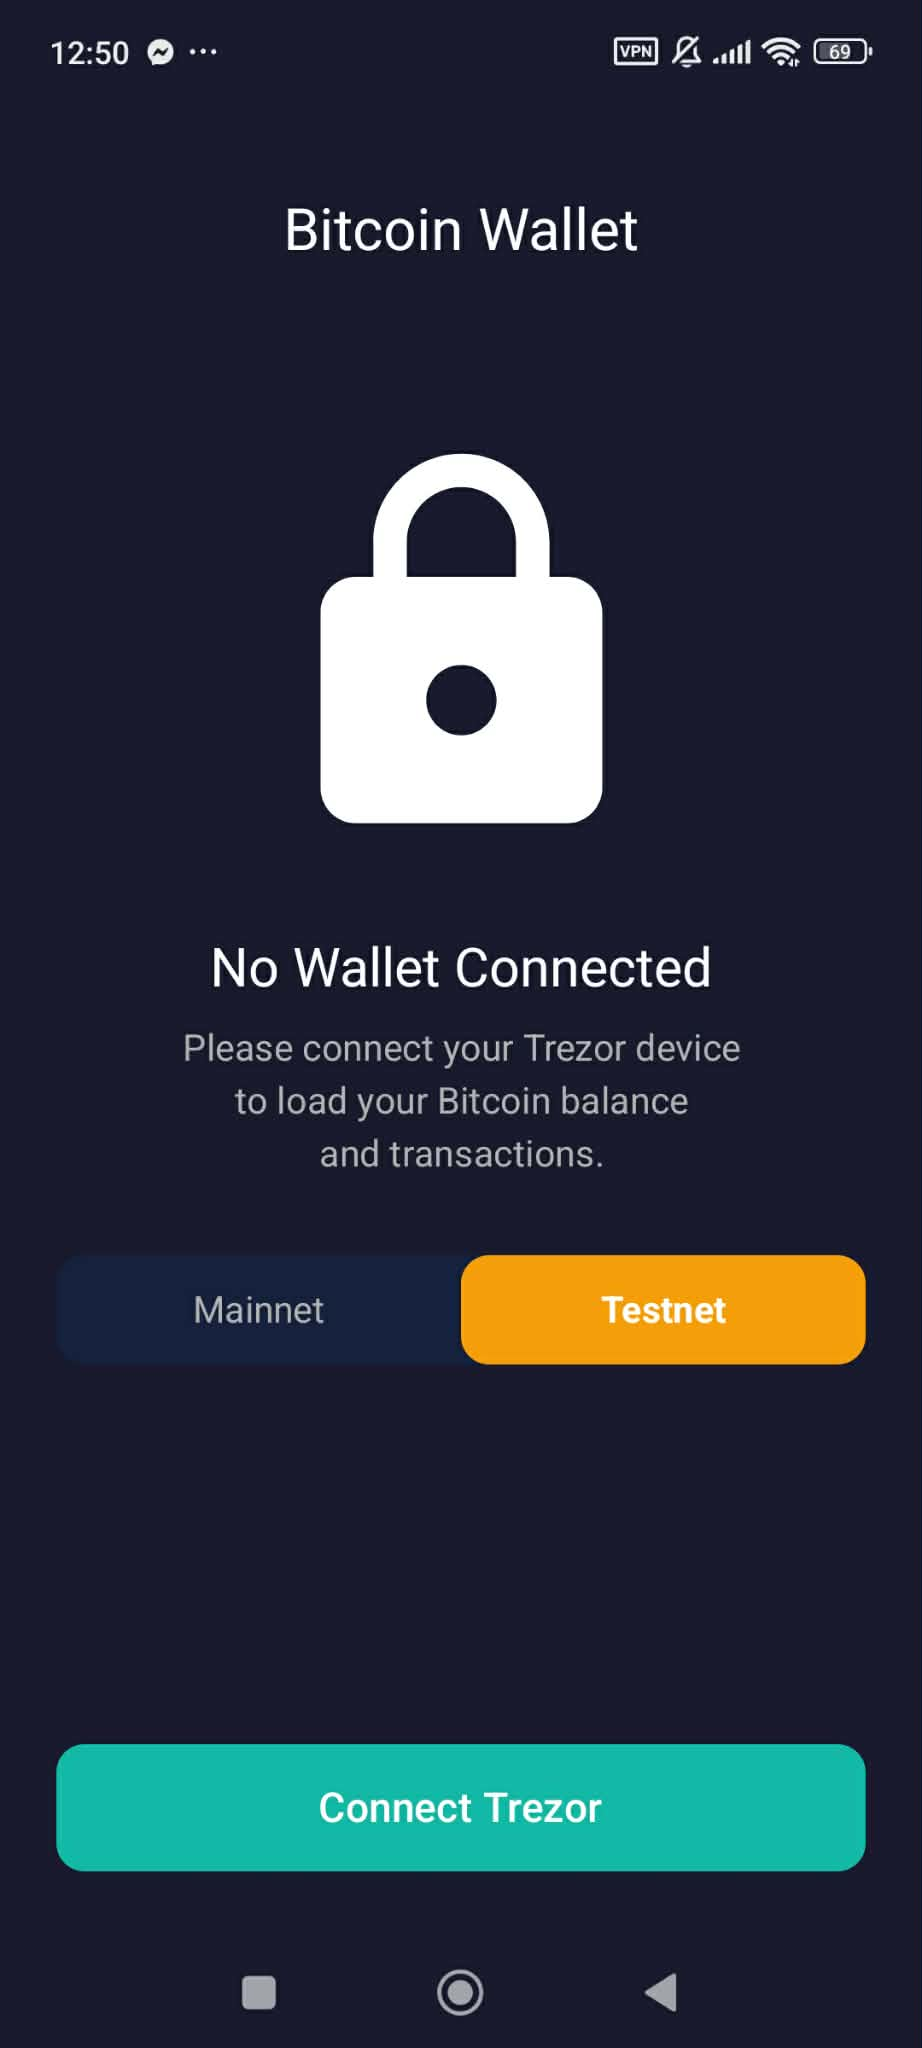
\includegraphics[height=0.3\textheight]{img/screen-login.jpeg}\hfill
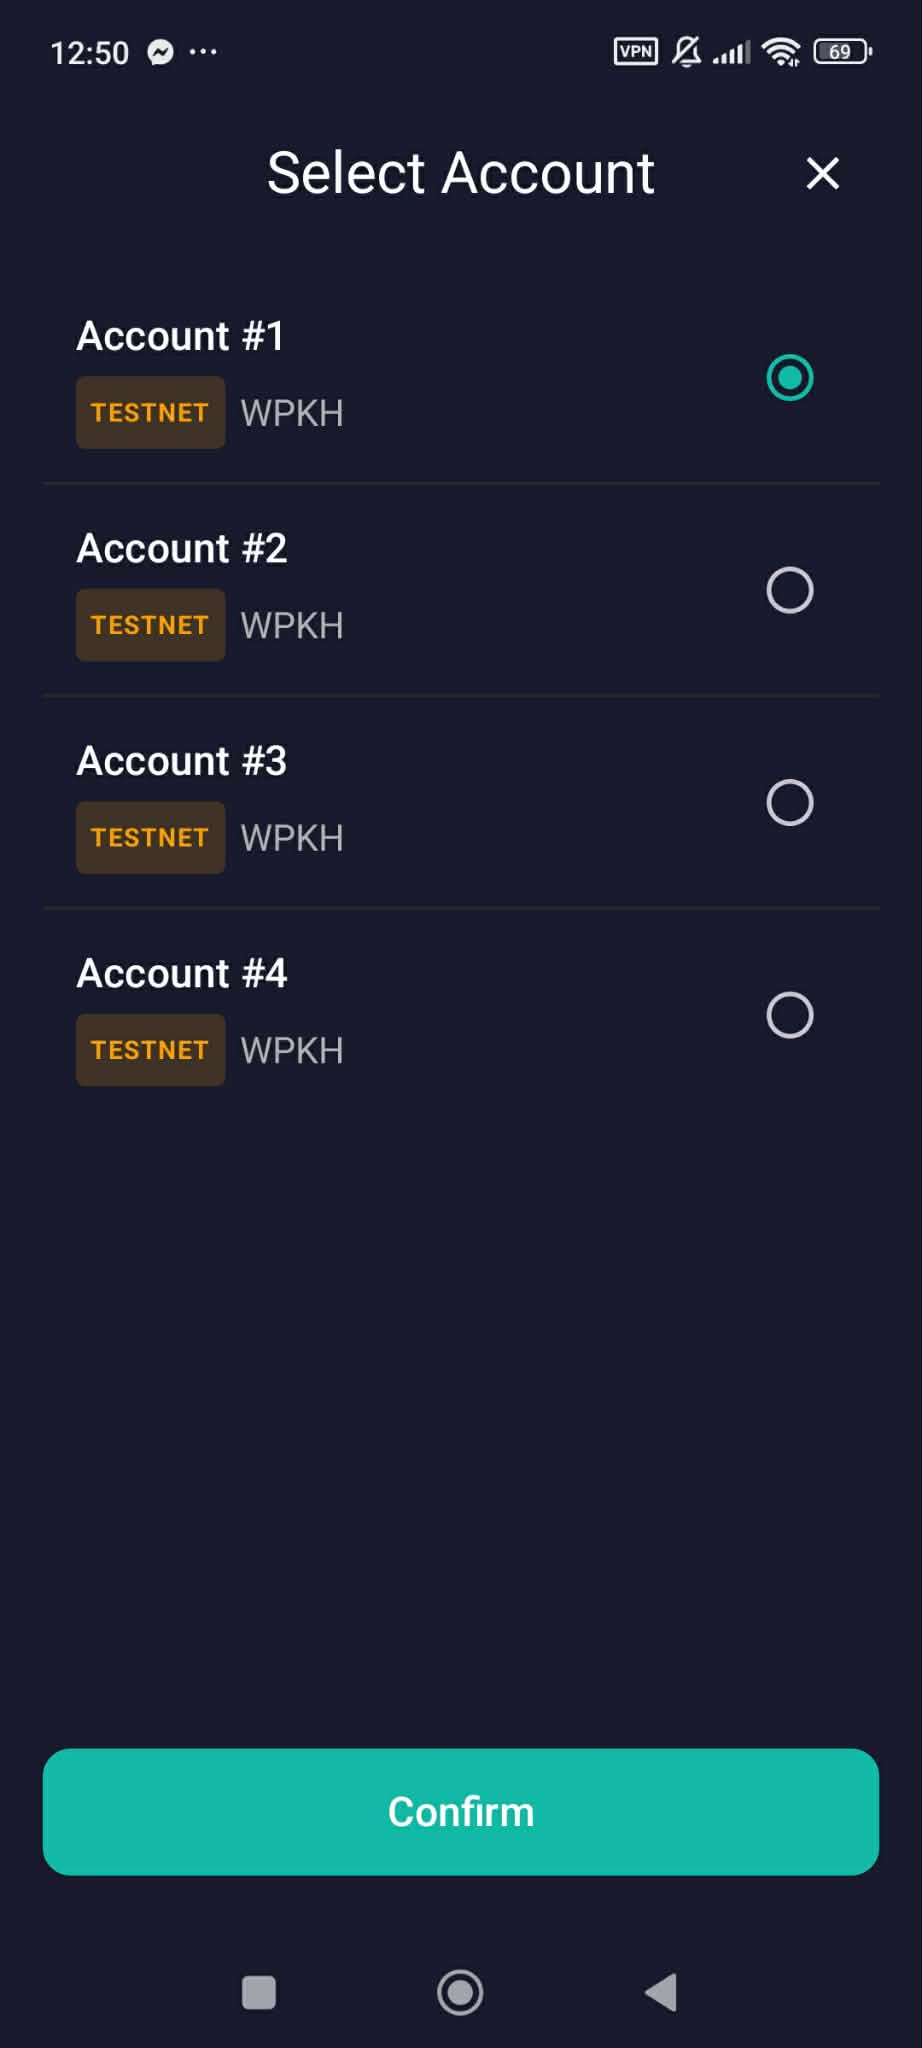
\includegraphics[height=0.3\textheight]{img/screen-select-account.jpeg}\hfill
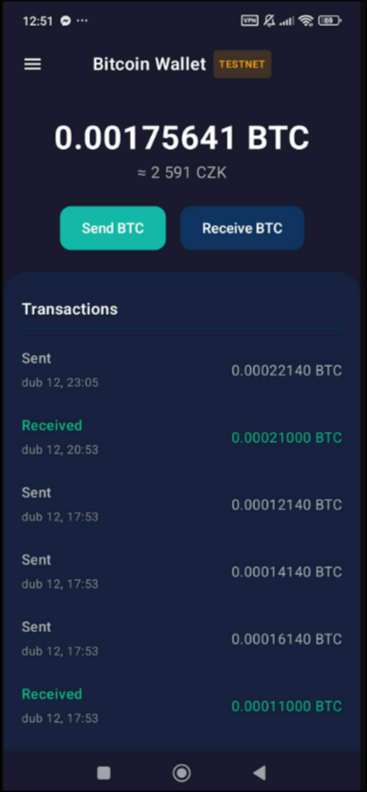
\includegraphics[height=0.3\textheight]{img/screen-dashboard.png}
\caption[Průběh přihlášení]{Průběh přihlášení. Vlevo: přihlašovací
obrazovka s~přepínačem sítě. Uprostřed: výběr singlesig účtu --
backend nalezl čtyři účty s~historií. Vpravo: hlavní obrazovka
(dashboard) se zůstatkem v~BTC a~CZK, seznamem transakcí a~tlačítky
pro odeslání a~příjem.}
\label{fig:screen-onboarding}
\end{figure}

Tento postup probíhá pouze při prvním přihlášení. V~běžném provozu
aplikace po~vypršení krátkodobého přístupového tokenu automaticky vymění
uchovávaný refresh token za~novou dvojici tokenů, aniž by uživatel
musel znovu exportovat klíče z~Trezoru; mechanismus rotace popisujeme
v~sekci~\ref{subsec:refresh-token}.

Hlavní obrazovka (dashboard) zobrazuje aktuální zůstatek v~BTC a~jeho
ekvivalent ve zvolené fiat měně (CZK, USD nebo EUR -- volbu měny lze
změnit v~nastavení aplikace, viz sekci~\ref{sec:user-nastaveni}). Pod
zůstatkem se nachází chronologický seznam transakcí seřazený od nejnovější;
u~každé transakce je uvedena částka, směr (odeslaná/přijatá), datum a~čas
nebo příznak \emph{Unconfirmed} u~dosud nepotvrzených transakcí. V~dolní části
obrazovky jsou dvě hlavní tlačítka: \emph{Send BTC} pro vytvoření nové
transakce a~\emph{Receive BTC} pro zobrazení přijímací adresy. V~levém
horním rohu ikona hamburgeru otevírá postranní navigační menu
(\emph{drawer}), které umožňuje přechod na seznam multisig peněženek
a~do nastavení. Kliknutím na konkrétní transakci v~seznamu se otevře její
detail (viz sekci~\ref{sec:user-detail-tx}).

%%% -----------------------------------------------------------------------
\section{Příjem prostředků}
\label{sec:user-prijem}

Po stisknutí \emph{Receive BTC} aplikace zobrazí aktuální přijímací adresu
(obrázek~\ref{fig:screen-receive}) ve formě řetězce \texttt{tb1q\ldots}
(na testnetu) nebo \texttt{bc1q\ldots} (na mainnetu) spolu
s~odpovídajícím QR kódem ve formátu BIP-21~\cite{BIP21} (URI ve tvaru
\texttt{bitcoin:<adresa>}). Adresu lze zkopírovat do schránky stisknutím
příslušného tlačítka.

Tlačítko \emph{Show On Trezor} umožňuje ověřit zobrazenou adresu přímo
na displeji hardwarové peněženky. Aplikace prostřednictvím deeplinku zavolá
metodu \texttt{getAddress} protokolu Trezor Connect~\cite{TrezorConnect}
a~Trezor na svém displeji zobrazí adresu odvozenou ze svých interních klíčů.
Uživatel vizuálně porovná obě adresy a~tím ověří, že aplikace nezobrazuje
podvrženou adresu. Tato funkce je dostupná jak pro singlesig, tak pro
multisig peněženky.

\begin{figure}[htbp]
\centering
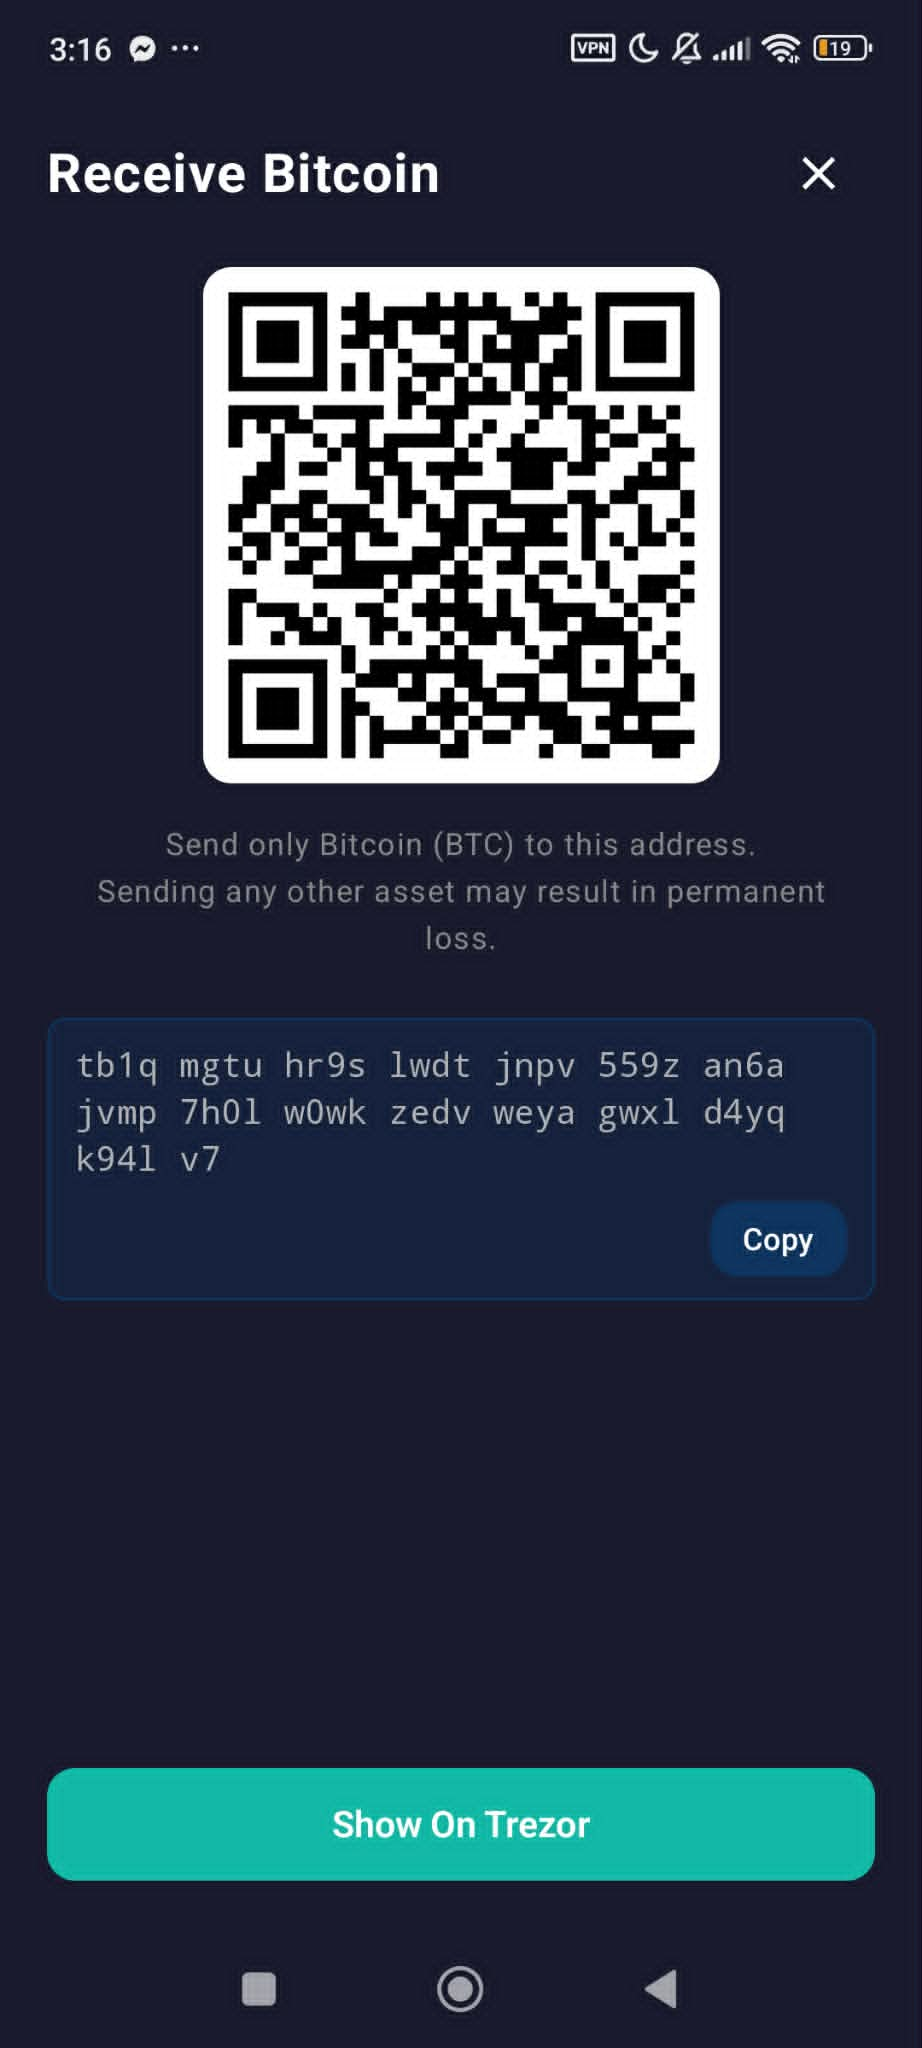
\includegraphics[height=0.3\textheight]{img/screen-receive.jpeg}
\caption[Příjem prostředků]{Příjem prostředků -- QR kód ve formátu
BIP-21, adresa s~možností kopírování a~tlačítko pro ověření adresy
na displeji Trezoru.}
\label{fig:screen-receive}
\end{figure}

Po přijetí prostředků na zobrazenou adresu se zůstatek
v~aplikaci aktualizuje po obnovení dashboardu; první potvrzení v~bloku
obvykle trvá 10--30 minut.

%%% -----------------------------------------------------------------------
\section{Odeslání singlesig transakce}
\label{sec:user-singlesig}

Po stisknutí \emph{Send BTC} se otevře formulář
(obrázek~\ref{fig:screen-send}) s~následujícími poli:

\begin{description}
\item[Cílová adresa] -- uživatel ji zadá ručně, vloží ze schránky, nebo
  naskenuje pomocí QR kódu z~fotoaparátu zařízení stisknutím ikony QR skeneru
  vedle pole adresy. Skener rozpozná jak prosté adresy, tak BIP-21
  URI~\cite{BIP21} ve tvaru \texttt{bitcoin:<adresa>} a~automaticky extrahuje
  samotnou adresu.

\item[Částka] -- zadává se v~BTC.

\item[Výběr UTXO] -- uživatel volí mezi automatickým výběrem (strategie
  \emph{largest-first}, viz sekci~\ref{subsec:coin-control}) a~manuálním
  výběrem (obrázek~\ref{fig:screen-send}, uprostřed). Při zvolení
  manuálního režimu se tlačítkem \emph{Edit} otevře obrazovka coin control
  (viz sekci~\ref{sec:user-coin-control}).

\item[Úroveň poplatku] -- výběr ze tří úrovní (nízký, střední, vysoký)
  s~aktuální sazbou v~sat/vB získanou z~mempoolu. V~manuálním režimu
  výběru UTXO je navíc dostupné pole pro zadání libovolné sazby ručně.
\end{description}

Pod formulářem se zobrazuje souhrn transakce: odesílaná částka, odhadovaný
poplatek, celková hodnota, aktuální zůstatek, prostředky rezervované
v~rozpracovaných PSBT (pokud existují) a~zbývající změna (change). Tím má
uživatel před potvrzením kompletní přehled o~dopadu transakce na svůj
zůstatek.

\begin{figure}[htbp]
\centering
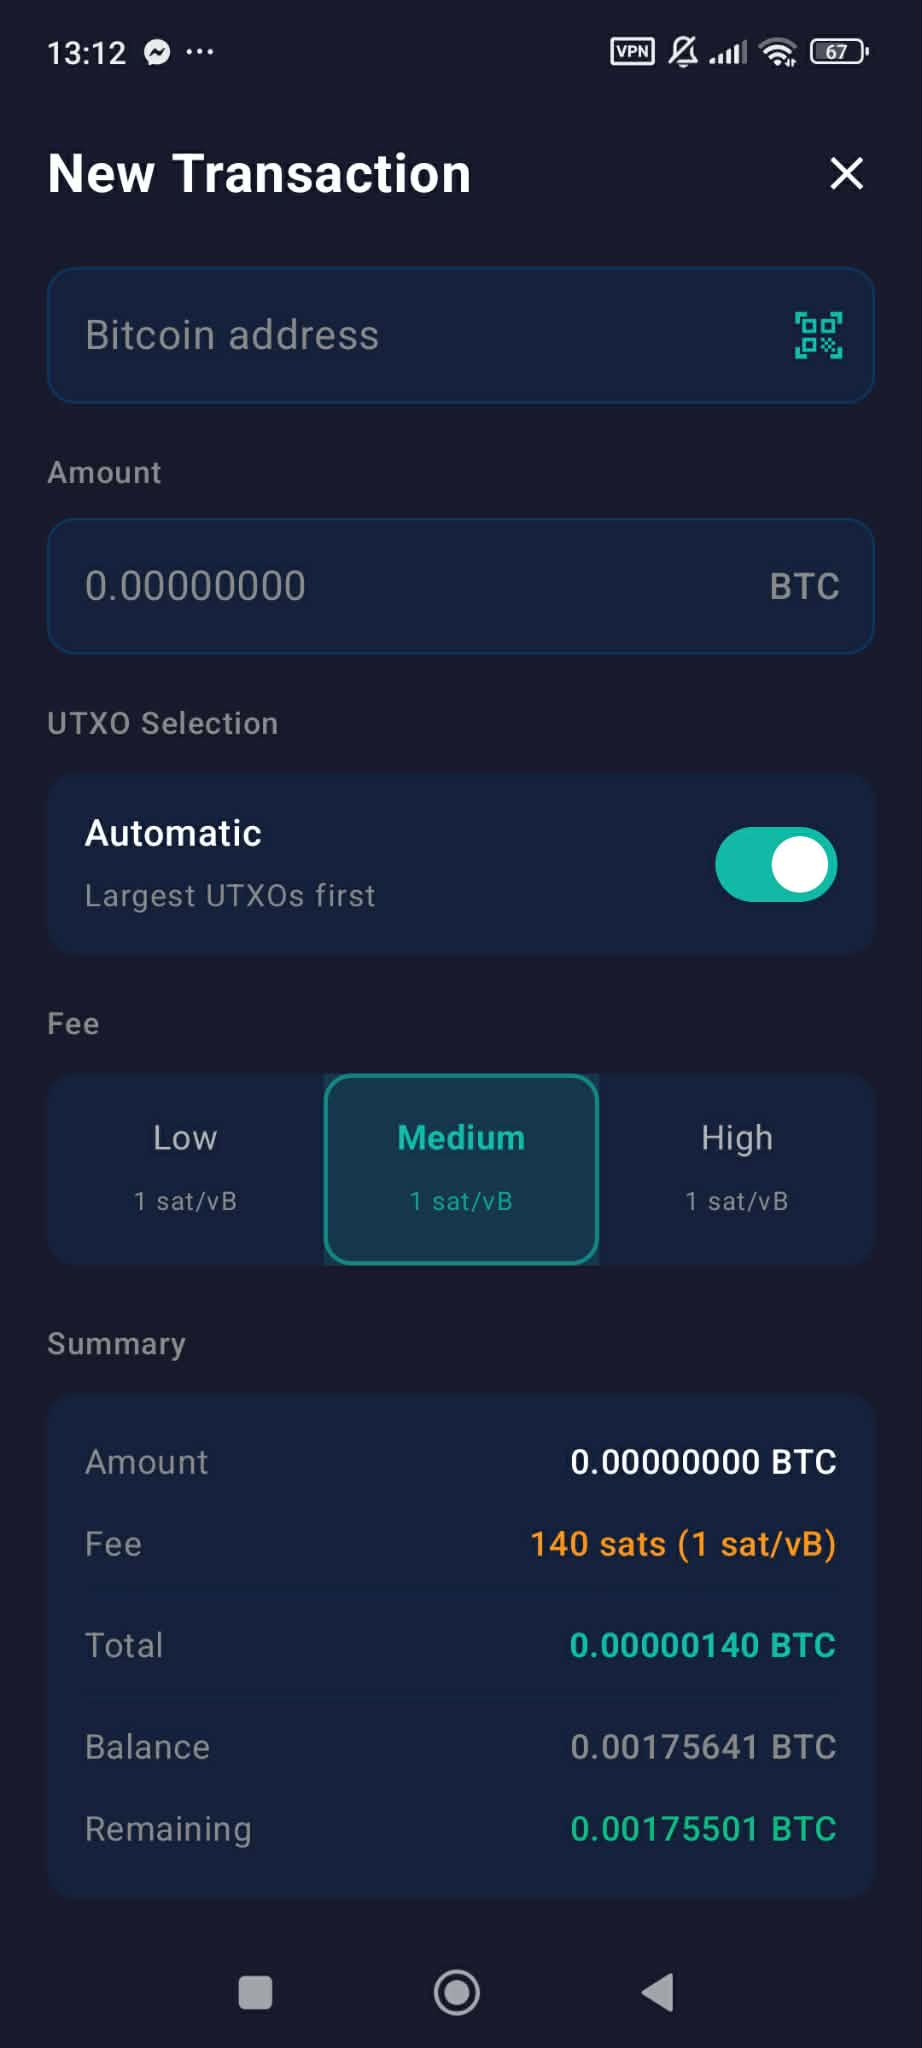
\includegraphics[height=0.3\textheight]{img/screen-send.jpeg}\hfill
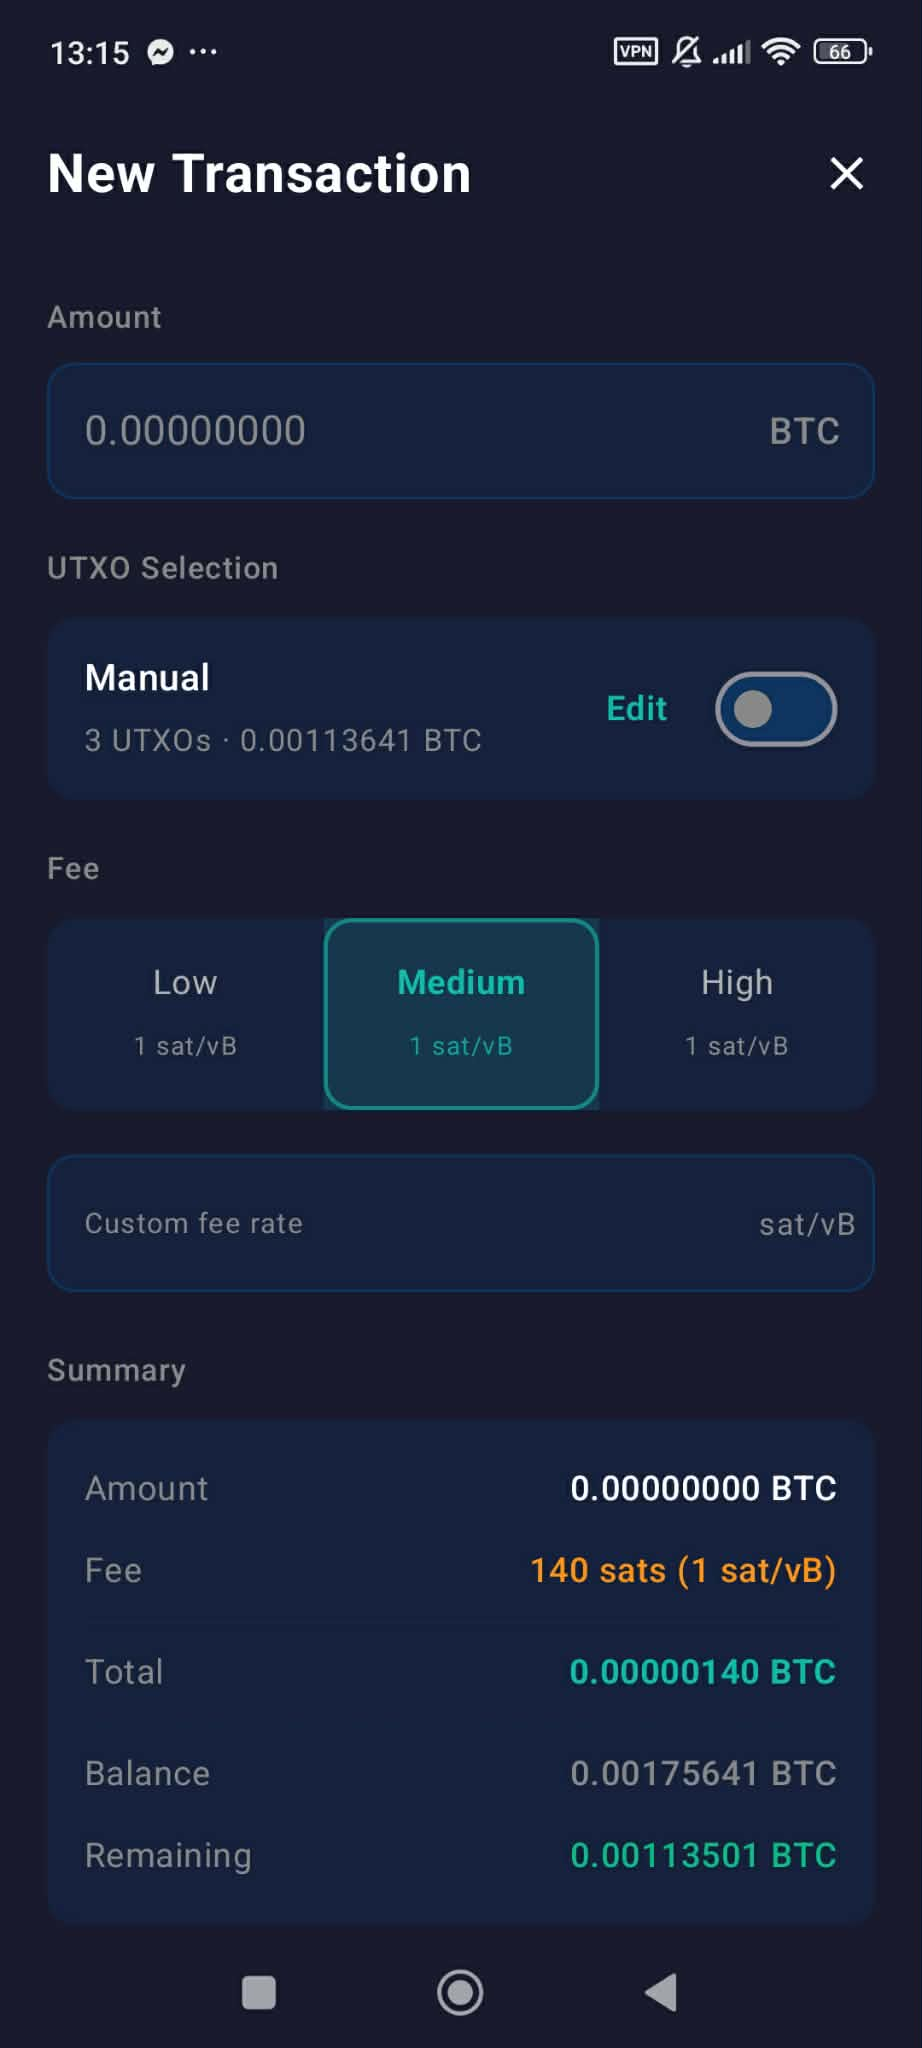
\includegraphics[height=0.3\textheight]{img/screen-send-manual.jpeg}\hfill
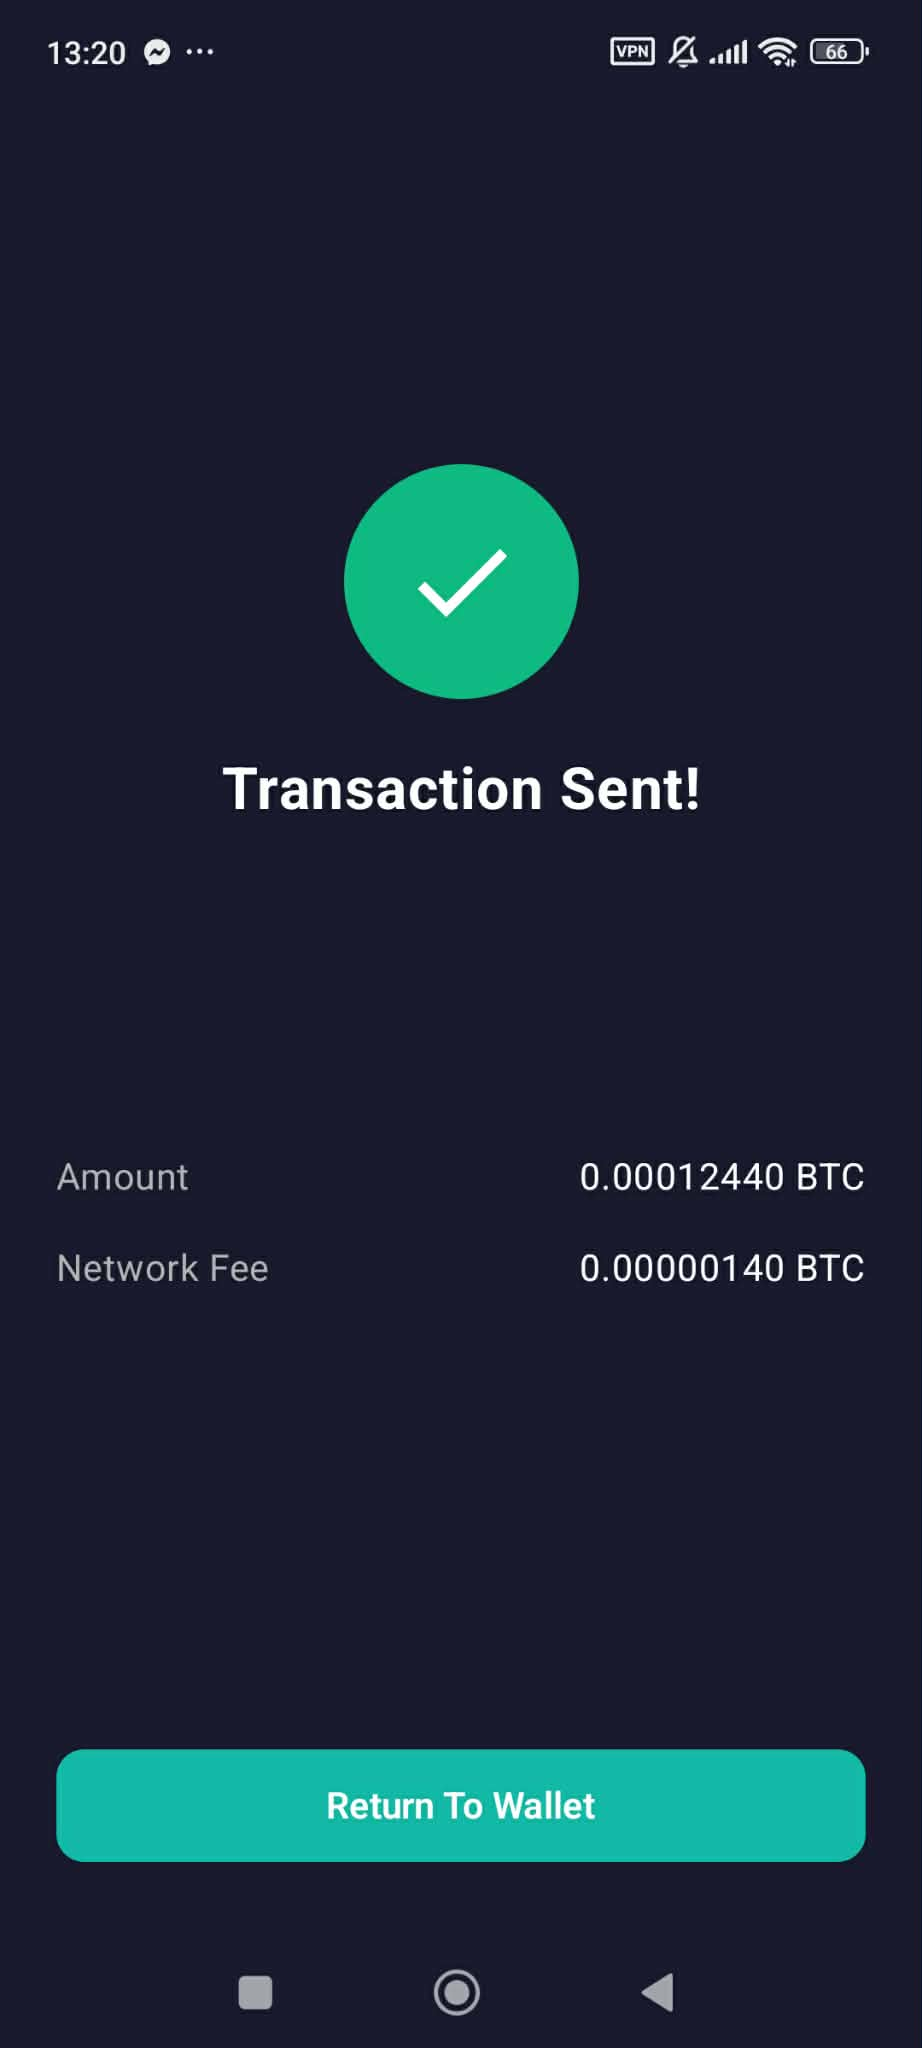
\includegraphics[height=0.3\textheight]{img/screen-tx-sent.jpeg}
\caption[Odeslání transakce]{Odeslání transakce. Vlevo: formulář
s~automatickým výběrem UTXO a~třemi úrovněmi poplatku. Uprostřed:
manuální režim s~počtem vybraných UTXO a~polem pro vlastní sazbu
v~sat/vB. Vpravo: potvrzení úspěšného odeslání se souhrnem částky
a~poplatku.}
\label{fig:screen-send}
\end{figure}

Po potvrzení odeslání backend sestaví transakci typu P2WPKH a~aplikace
přes deeplink přesměruje uživatele do Trezor Suite Mobile. Tam se
na displeji hardwarové peněženky zobrazí cílová adresa, částka a~poplatek
ke kontrole; uživatel podpis fyzicky potvrdí stisknutím tlačítka na
zařízení. Trezor vrátí kompletní podepsanou transakci, kterou aplikace
předá backendu k~broadcastu do Bitcoinové sítě. Po úspěšném broadcastu
aplikace zobrazí potvrzení s~částkou a~poplatkem
(obrázek~\ref{fig:screen-send}, vpravo),
podle kterého lze průběh sledovat v~kterémkoli prohlížeči blockchainu.
V~případě neúspěchu (například odmítnutí podpisu na Trezoru nebo chyba
sítě) se zobrazí chybová obrazovka s~popisem problému a~tlačítkem pro
návrat na dashboard.

%%% -----------------------------------------------------------------------
\section{Manuální výběr UTXO (coin control)}
\label{sec:user-coin-control}

Obrazovka coin control (obrázek~\ref{fig:screen-tools}, vlevo) zobrazuje
seznam všech nepoužitých výstupů (UTXO) aktuální peněženky. U~každého UTXO
je uvedena částka v~BTC, adresa, datum vytvoření a~stav:

\begin{description}
\item[Potvrzený] (zelený příznak) -- UTXO je potvrzeno v~alespoň jednom
  bloku a~je k~dispozici pro výběr.
\item[Nepotvrzený] (žlutý příznak) -- UTXO pochází z~transakce, která
  dosud nebyla zařazena do bloku. Je k~dispozici pro výběr, ale transakce
  využívající nepotvrzený vstup může být zpožděna.
\item[Rezervovaný] (červený příznak) -- UTXO je zamčeno v~rozpracované
  PSBT transakci čekající na podpisy. Takové UTXO nelze vybrat, aby se
  předešlo dvojímu utracení.
\end{description}

Uživatel zaškrtne konkrétní UTXO, která chce použít jako vstupy transakce.
V~horní části obrazovky se průběžně zobrazuje počet vybraných UTXO
a~jejich celková hodnota. Tlačítkem \emph{Order By} je možné změnit řazení
seznamu podle hodnoty, data, stavu potvrzení nebo adresy.

Kliknutím na obsah řádku UTXO (nikoliv na zaškrtávací pole) se otevře
detail příslušné transakce (viz sekci~\ref{sec:user-detail-tx}), kde
uživatel může prozkoumat původ prostředků.

%%% -----------------------------------------------------------------------
\section{Detail transakce}
\label{sec:user-detail-tx}

Obrazovka detailu transakce (obrázek~\ref{fig:screen-tools}, uprostřed)
zobrazuje kompletní informace o~zvolené transakci: stav potvrzení
(potvrzená s~výškou bloku, nebo nepotvrzená), časové razítko, poplatek
v~BTC, sazbu poplatku v~sat/vB a~velikost transakce v~bajtech.

Pod hlavičkou se nachází dva seznamy: vstupy a~výstupy transakce. U~každého
vstupu a~výstupu je zobrazena adresa, hodnota v~BTC a~barevné příznaky:
\emph{YOURS} označuje adresu patřící aktuální peněžence a~\emph{FROM HERE}
zvýrazňuje výstup, z~něhož uživatel na tuto transakci přišel (při
rekurzivním procházení). Kliknutím na vstup nebo výstup se otevře detailní
dialog zobrazující plnou adresu, hodnotu v~BTC i~v~satoshi a~v~případě
vstupu i~identifikátor předchozí transakce s~tlačítkem
\emph{Open previous transaction}.

Tímto tlačítkem uživatel otevře předchozí transakci odpovídající danému
vstupu, čímž může rekurzivně sledovat původ prostředků. Aktuální hloubku
průchodu zobrazuje indikátor v~záhlaví (například \uv{Depth 2~/~5}). Aby
nedošlo k~nadměrnému zatížení blockchainového API, je hloubka průchodu
omezena na pět úrovní; po dosažení limitu se zobrazí upozornění. Tlačítko
\emph{Zavřít} v~horní části obrazovky vrátí uživatele zpět na dashboard
bez ohledu na aktuální hloubku průchodu.

\begin{figure}[htbp]
\centering
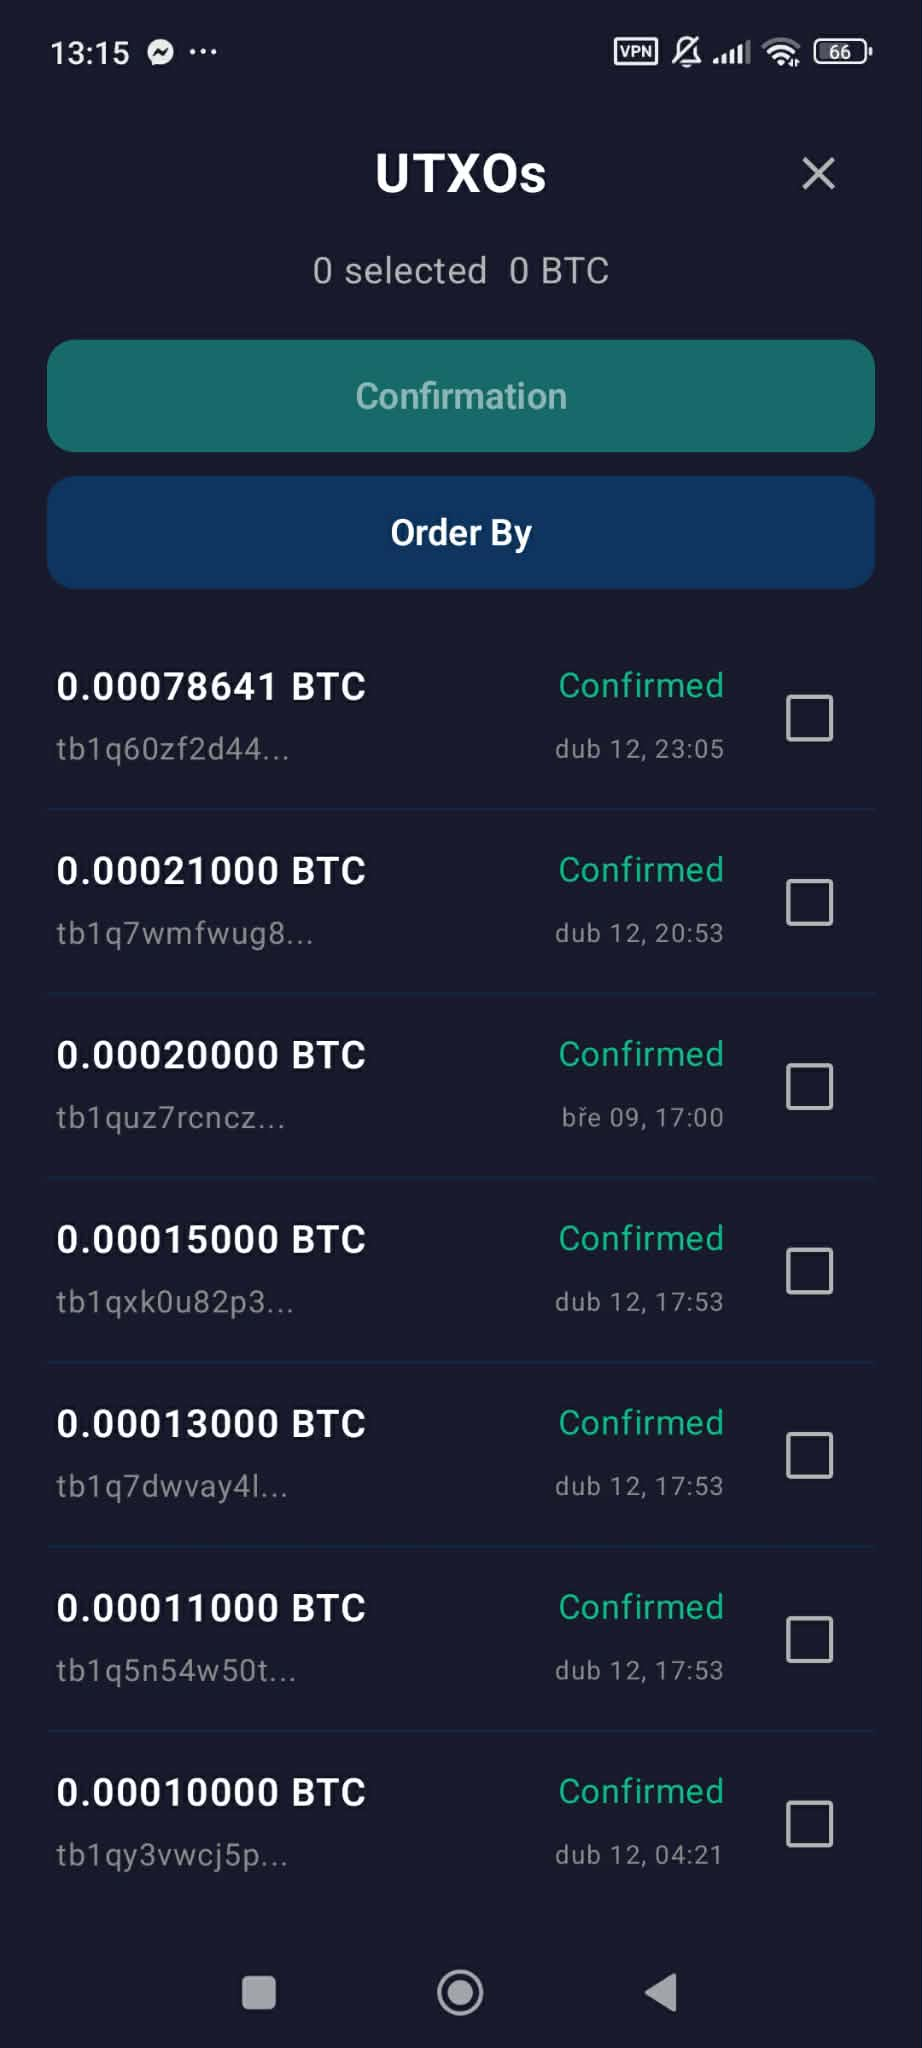
\includegraphics[height=0.3\textheight]{img/screen-coin-control.jpeg}\hfill
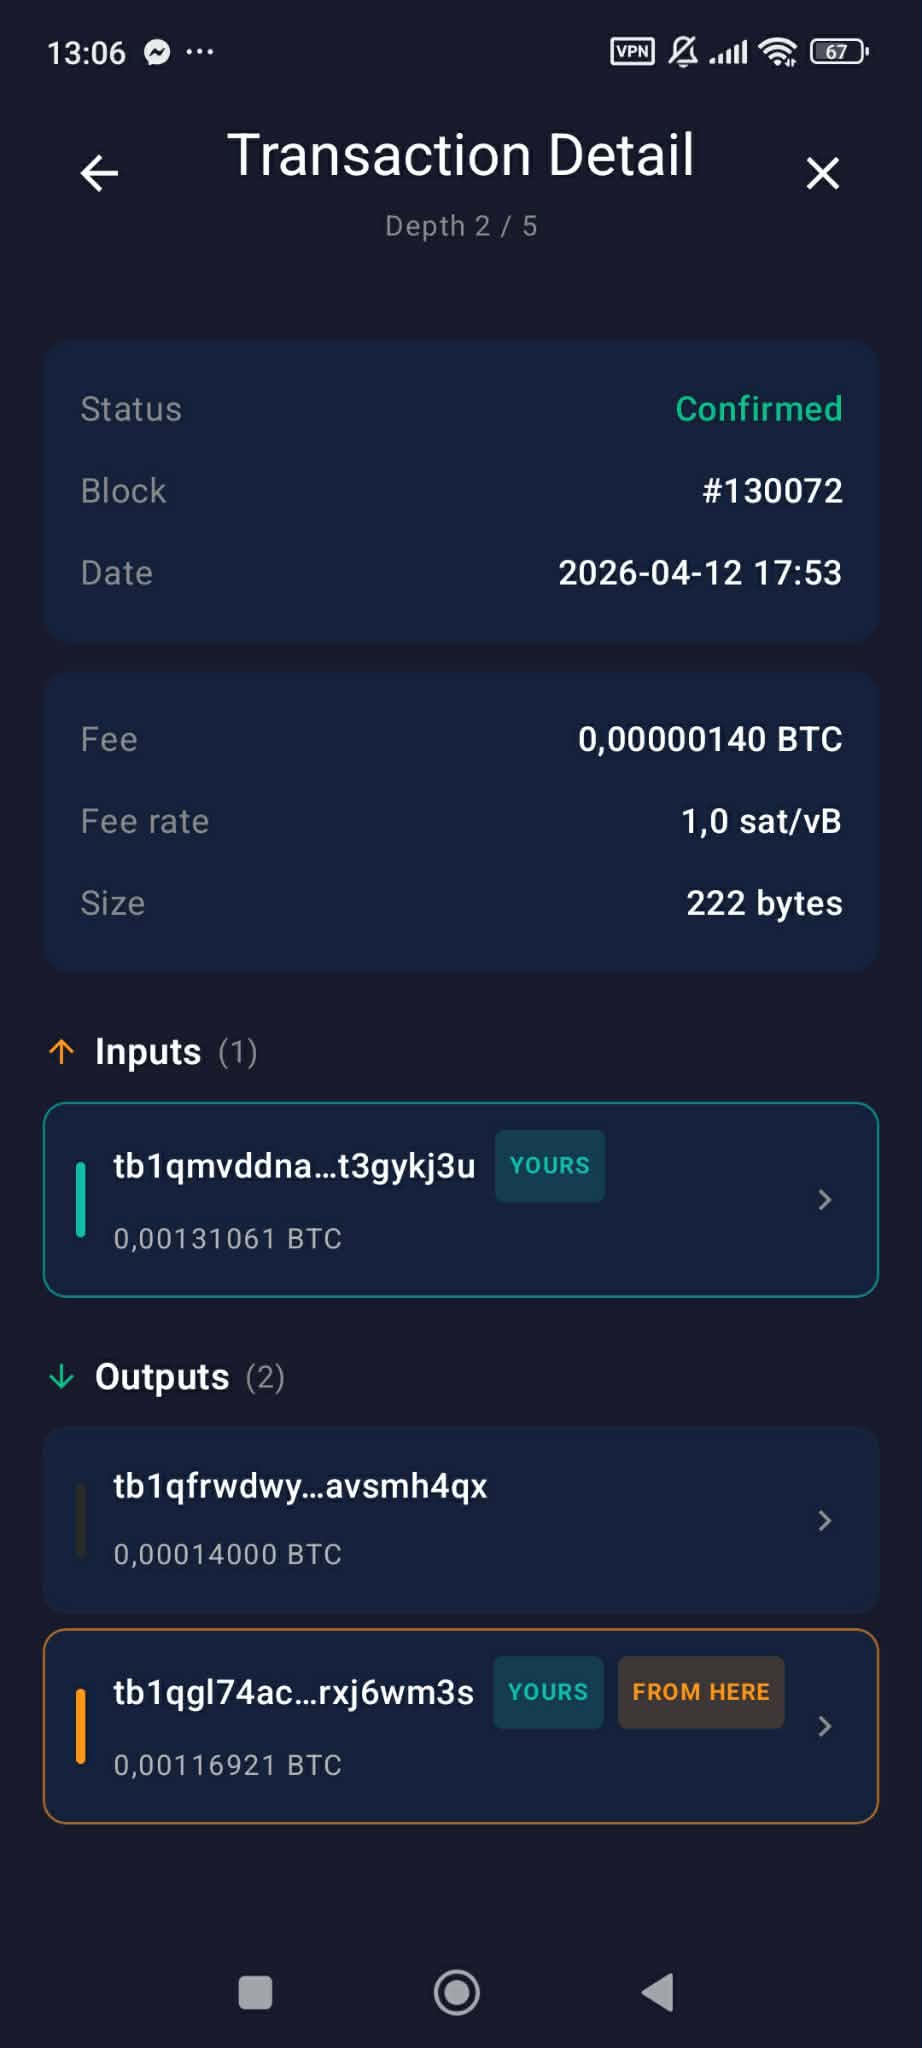
\includegraphics[height=0.3\textheight]{img/screen-tx-detail.jpeg}\hfill
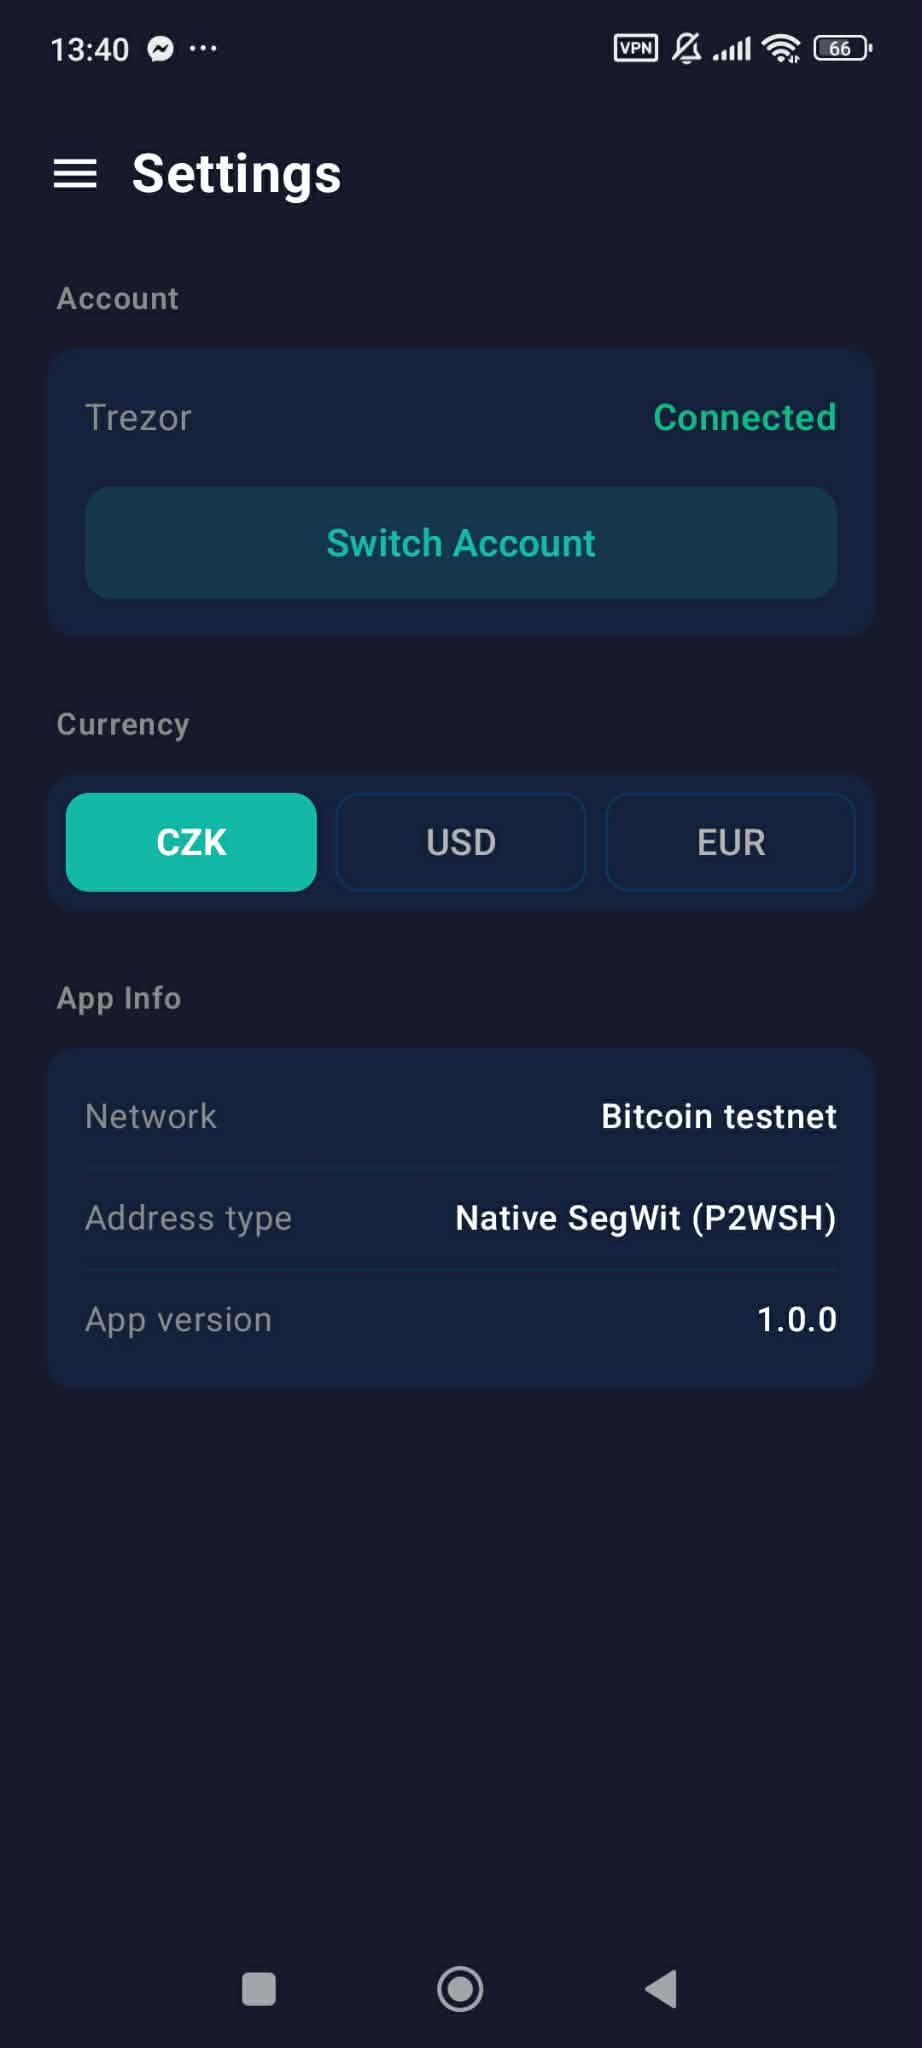
\includegraphics[height=0.3\textheight]{img/screen-settings.jpeg}
\caption[Coin control, detail transakce a nastavení]{Vlevo: coin
control -- seznam UTXO s~hodnotou, adresou, datem a~stavem potvrzení.
Uprostřed: detail transakce v~hloubce 2\,/\,5 s~příznaky \emph{YOURS}
a~\emph{FROM HERE}. Vpravo: nastavení -- přepnutí účtu, výběr fiat
měny a~informace o~aplikaci.}
\label{fig:screen-tools}
\end{figure}

%%% -----------------------------------------------------------------------
\section{Nastavení}
\label{sec:user-nastaveni}

Obrazovka nastavení (obrázek~\ref{fig:screen-tools}, vpravo) je přístupná
z~postranního navigačního menu a~obsahuje následující funkce:

\begin{description}
\item[Přepnout účet] -- smaže aktuální výběr peněženky a~přesměruje
  uživatele zpět na obrazovku výběru účtu. V~kontextu multisig testování
  (popsaného v~sekci~\ref{sec:user-multisig-podpis}) umožňuje přepínat
  mezi různými BIP-48 účty na témže Trezoru, čímž uživatel simuluje
  různé cosignery.

\item[Fiat měna] -- přepínač umožňující zvolit měnu pro zobrazení
  ekvivalentní hodnoty zůstatku: česká koruna (CZK), americký dolar (USD)
  nebo euro (EUR). Volba se projeví na dashboardu i~na detailu multisig
  peněženky. Směnný kurz je poskytován službou \texttt{price-service},
  která jej získává z~CoinGecko API~\cite{CoinGeckoAPI}.

\item[Informace o~aplikaci] -- zobrazuje síť (Bitcoin mainnet/testnet),
  typ adres (Native SegWit) a~verzi aplikace.
\end{description}

%%% -----------------------------------------------------------------------
\section{Multisig peněženky}
\label{sec:user-multisig}

Práce s~multisig peněženkou probíhá ve dvou fázích: jednorázový import
existujícího deskriptoru a~opakované podepisování konkrétních transakcí
postupně více cosignery.

\subsection{Import deskriptoru}
\label{sec:user-import}

Multisig peněženka se v~aplikaci vytvoří importem výstupního deskriptoru
ve formátu \texttt{wsh(sortedmulti(M,\ldots))} podle BIP-380~\cite{BIP380}
a~BIP-383~\cite{BIP383}. Deskriptor obsahuje práh~$M$, seznam xpub klíčů
všech cosignerů a~jejich derivační cesty. Podrobný popis formátu uvádíme
v~sekci~\ref{sec:descriptors}.

V~praxi předpokládáme, že deskriptor vytvoří jeden z~cosignerů
v~desktopové aplikaci -- nejčastěji Sparrow Wallet~\cite{SparrowWallet} --,
ze své instance Trezoru exportuje xpub a~od ostatních cosignerů obdrží
jejich xpub klíče stejným způsobem. Sparrow z~těchto klíčů vygeneruje
hotový deskriptor, který následně cosigneři předají všem členům multisig
peněženky (například skrze e-mail nebo sdílený dokument). Deskriptor
neobsahuje žádné soukromé údaje, takže jeho přenos nepředstavuje
bezpečnostní riziko.

V~mobilní aplikaci uživatel přejde z~postranního menu na seznam multisig
peněženek a~stiskne tlačítko \emph{Import Wallet}. Na importní obrazovce
(obrázek~\ref{fig:screen-multisig-setup}, vlevo) jsou k~dispozici dva
způsoby zadání deskriptoru:

\begin{enumerate}
\item \textbf{Vložení textu} -- uživatel zkopíruje deskriptor ze schránky
  do textového pole. Tento způsob je vhodný, pokud deskriptor obdržel
  například e-mailem nebo v~textové zprávě.

\item \textbf{Skenování QR kódu} -- stisknutím ikony QR skeneru vedle
  textového pole se otevře fotoaparát. Aplikace podporuje jak jednoduché
  QR kódy s~textovým deskriptorem, tak animované vícesnímkové QR kódy
  ve formátu UR (\emph{Uniform Resources})~\cite{BCR2020005}. Formát UR
  rozděluje dlouhá data do~sekvence menších QR kódů, které se postupně
  zobrazují na obrazovce zdrojového zařízení; aplikace je snímá
  průběžně a~zobrazuje ukazatel postupu (například \uv{Čtení QR\ldots{}
  65\,\%}). Tento formát používají airgap peněženky jako Keystone
  nebo Passport a~podporuje jej i~Sparrow Wallet pro export
  deskriptorů bez nutnosti síťového připojení.
\end{enumerate}

Volitelně může uživatel zadat pojmenování peněženky (například
\uv{Rodinná pokladna}). Backend deskriptor parsuje, odvodí přijímací
a~change adresy a~ověří jejich historii v~blockchainu. Po dokončení se nově
importovaná peněženka zobrazí v~seznamu multisig peněženek
(obrázek~\ref{fig:screen-multisig-setup}, uprostřed) s~označením prahu
(například \uv{2-of-3}) a~aktuálním zůstatkem.

\begin{figure}[htbp]
\centering
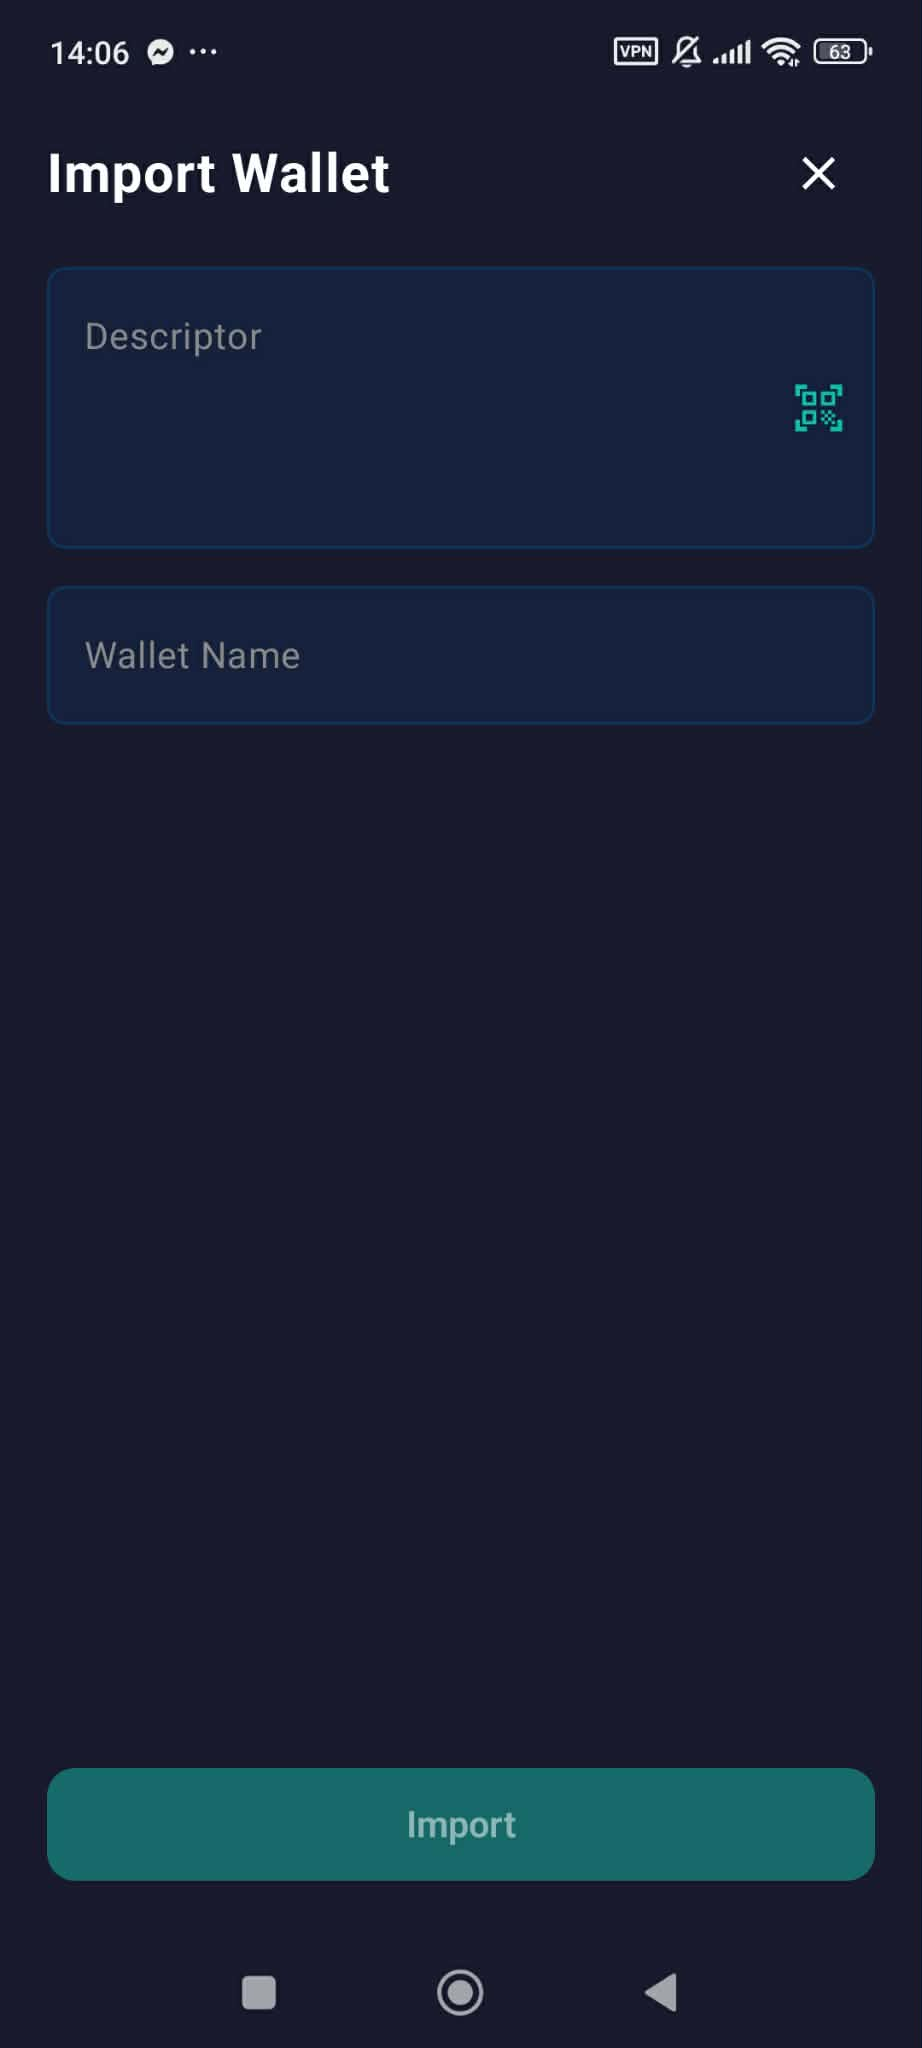
\includegraphics[height=0.3\textheight]{img/screen-import.jpeg}\hfill
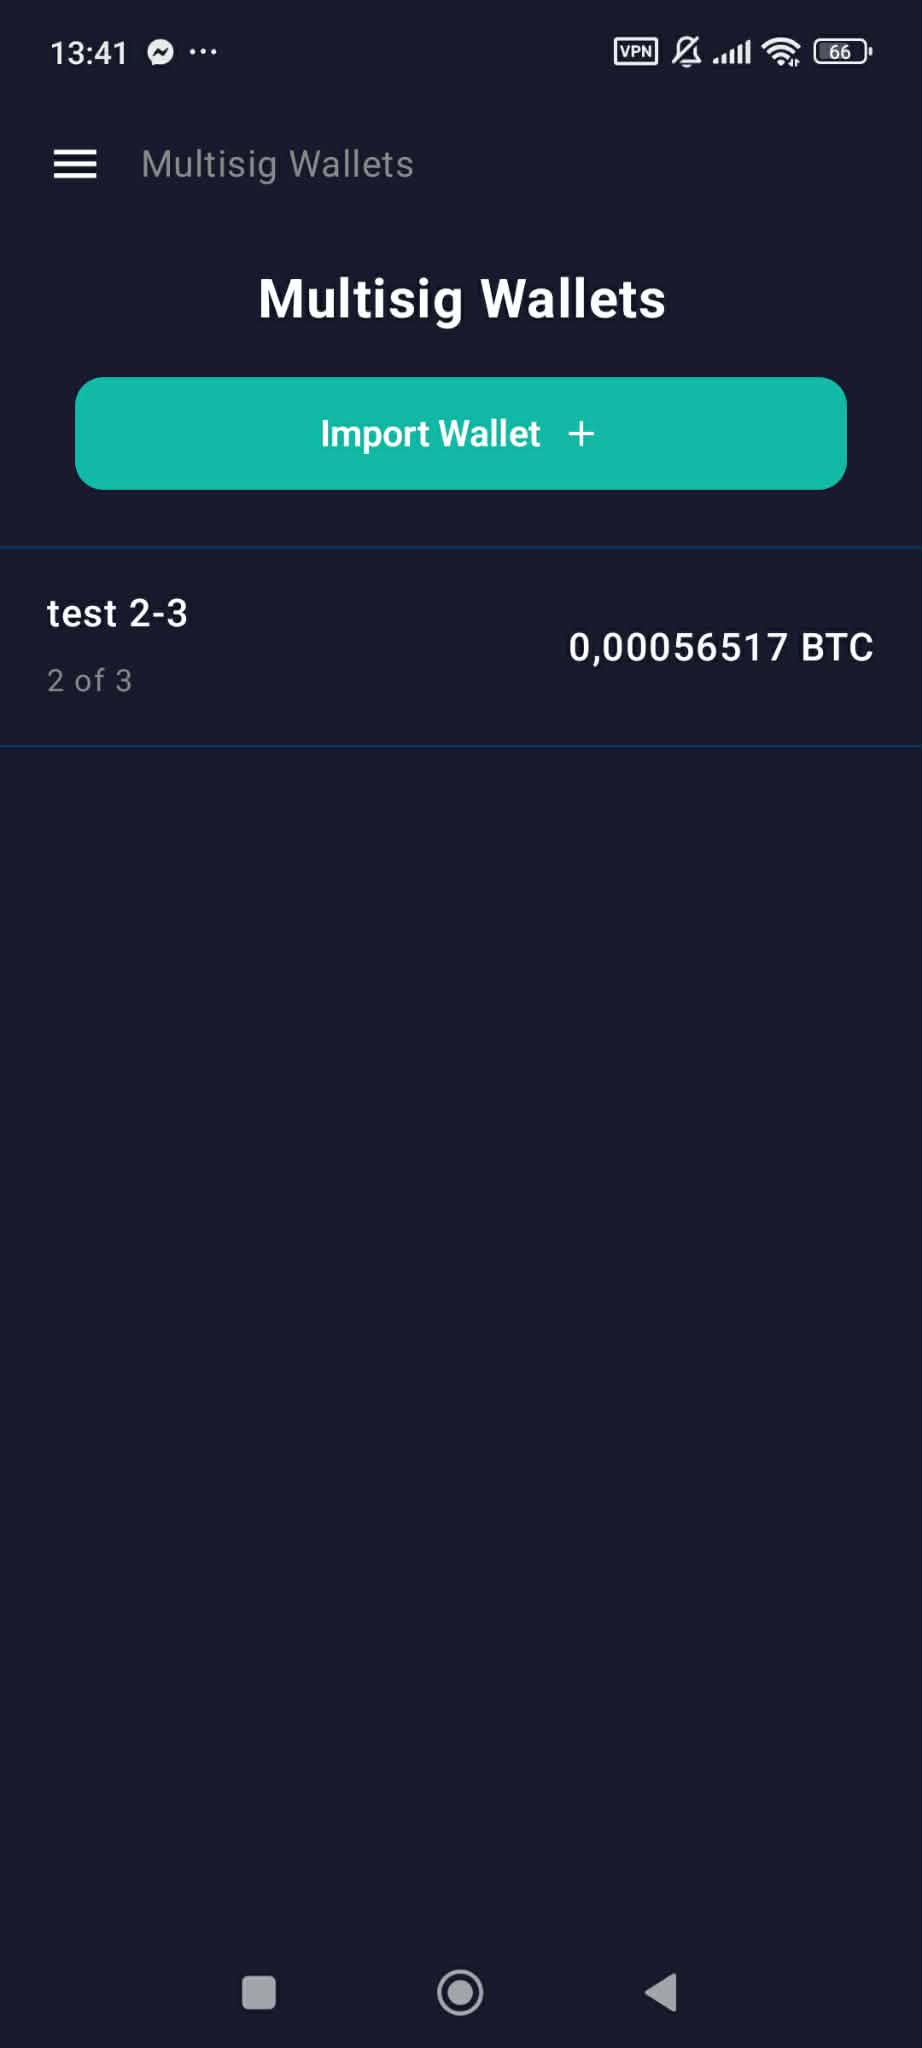
\includegraphics[height=0.3\textheight]{img/screen-multisig-list.jpeg}\hfill
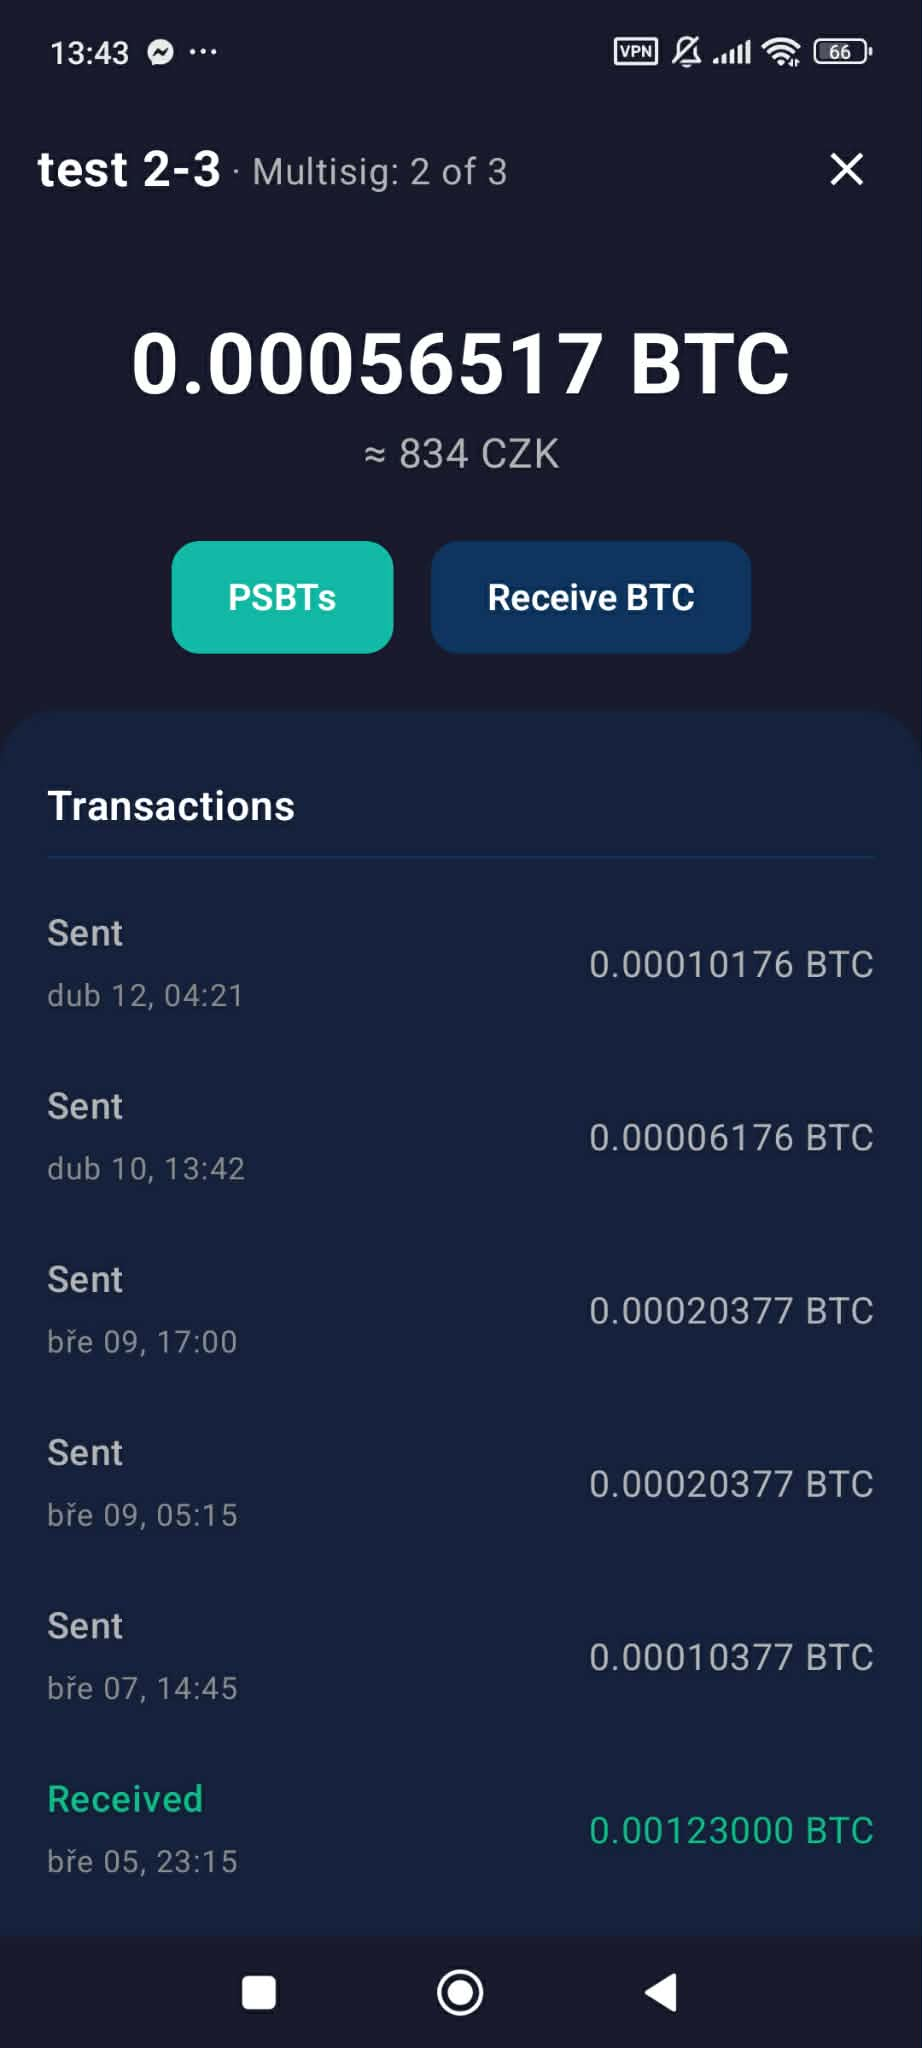
\includegraphics[height=0.3\textheight]{img/screen-multisig-detail.jpeg}
\caption[Multisig peněženky -- import a detail]{Multisig peněženky.
Vlevo: import deskriptoru s~ikonou QR skeneru a~pojmenováním.
Uprostřed: seznam importovaných multisig peněženek. Vpravo: detail
peněženky 2-of-3 se zůstatkem, historií transakcí a~přístupem
k~seznamu PSBT.}
\label{fig:screen-multisig-setup}
\end{figure}

\subsection{Seznam a detail multisig peněženky}

Po přechodu do sekce multisig peněženek z~postranního menu se zobrazí
seznam všech importovaných multisig peněženek přidružených k~aktuálnímu
účtu (obrázek~\ref{fig:screen-multisig-setup}, uprostřed). U~každé
peněženky je uveden její název, schéma (například 2-of-3) a~aktuální
zůstatek v~BTC.

Kliknutím na peněženku se otevře její detail
(obrázek~\ref{fig:screen-multisig-setup}, vpravo) -- obrazovka obdobná
dashboardu singlesig peněženky se zůstatkem (v~BTC i~ve fiat měně),
seznamem transakcí a~dvěma tlačítky: \emph{PSBTs} pro přechod na seznam
rozpracovaných transakcí a~\emph{Receive BTC} pro zobrazení přijímací
adresy (s~možností ověření na Trezoru).

\subsection{Vytvoření a podepsání multisig transakce}
\label{sec:user-multisig-podpis}

Vytvoření multisig transakce začíná na seznamu PSBT zvolené multisig
peněženky (obrázek~\ref{fig:screen-psbt-flow}, vlevo) stisknutím tlačítka
\emph{Create New PSBT}. Otevře se formulář shodný s~formulářem pro
singlesig odeslání (sekce~\ref{sec:user-singlesig}) -- uživatel zadá
cílovou adresu, částku a~úroveň poplatku. Backend však místo kompletní
transakce sestaví PSBT podle BIP-174~\cite{BIP174}, který kromě nepodepsané
transakce obsahuje i~derivační cesty cosignerů a~witness skript multisig
adresy. Aplikace poté přes deeplink přesměruje uživatele do Trezor Suite
Mobile k~podpisu na zařízení.

Trezor v~multisig režimu nevrací kompletní podepsanou transakci, ale pouze
pole podpisů odpovídajících danému cosignerovi. Backend tyto podpisy
přidá do PSBT na pozici, která odpovídá pořadí cosignera ve witness skriptu
podle BIP-67~\cite{BIP67}, a~uloží stav PSBT jako \uv{1 z~$M$ podpisů}.

\begin{figure}[htbp]
\centering
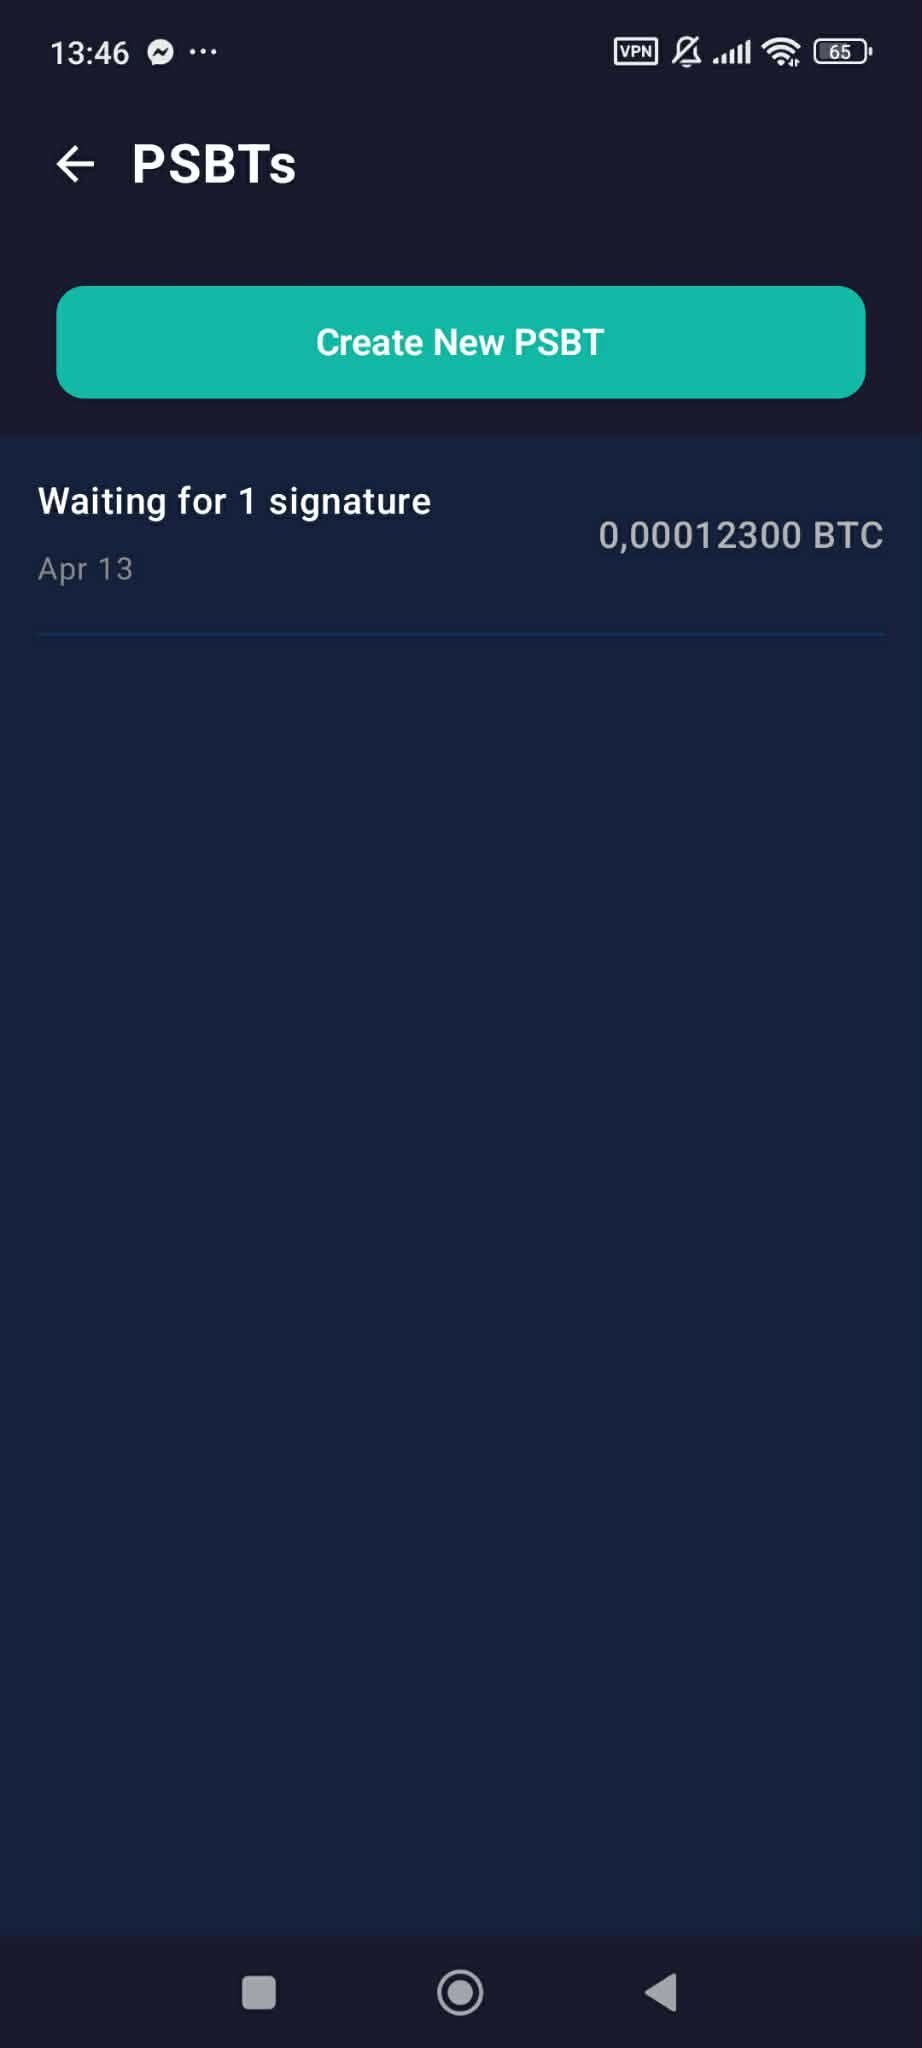
\includegraphics[height=0.22\textheight]{img/screen-psbt-list.jpeg}\hfill
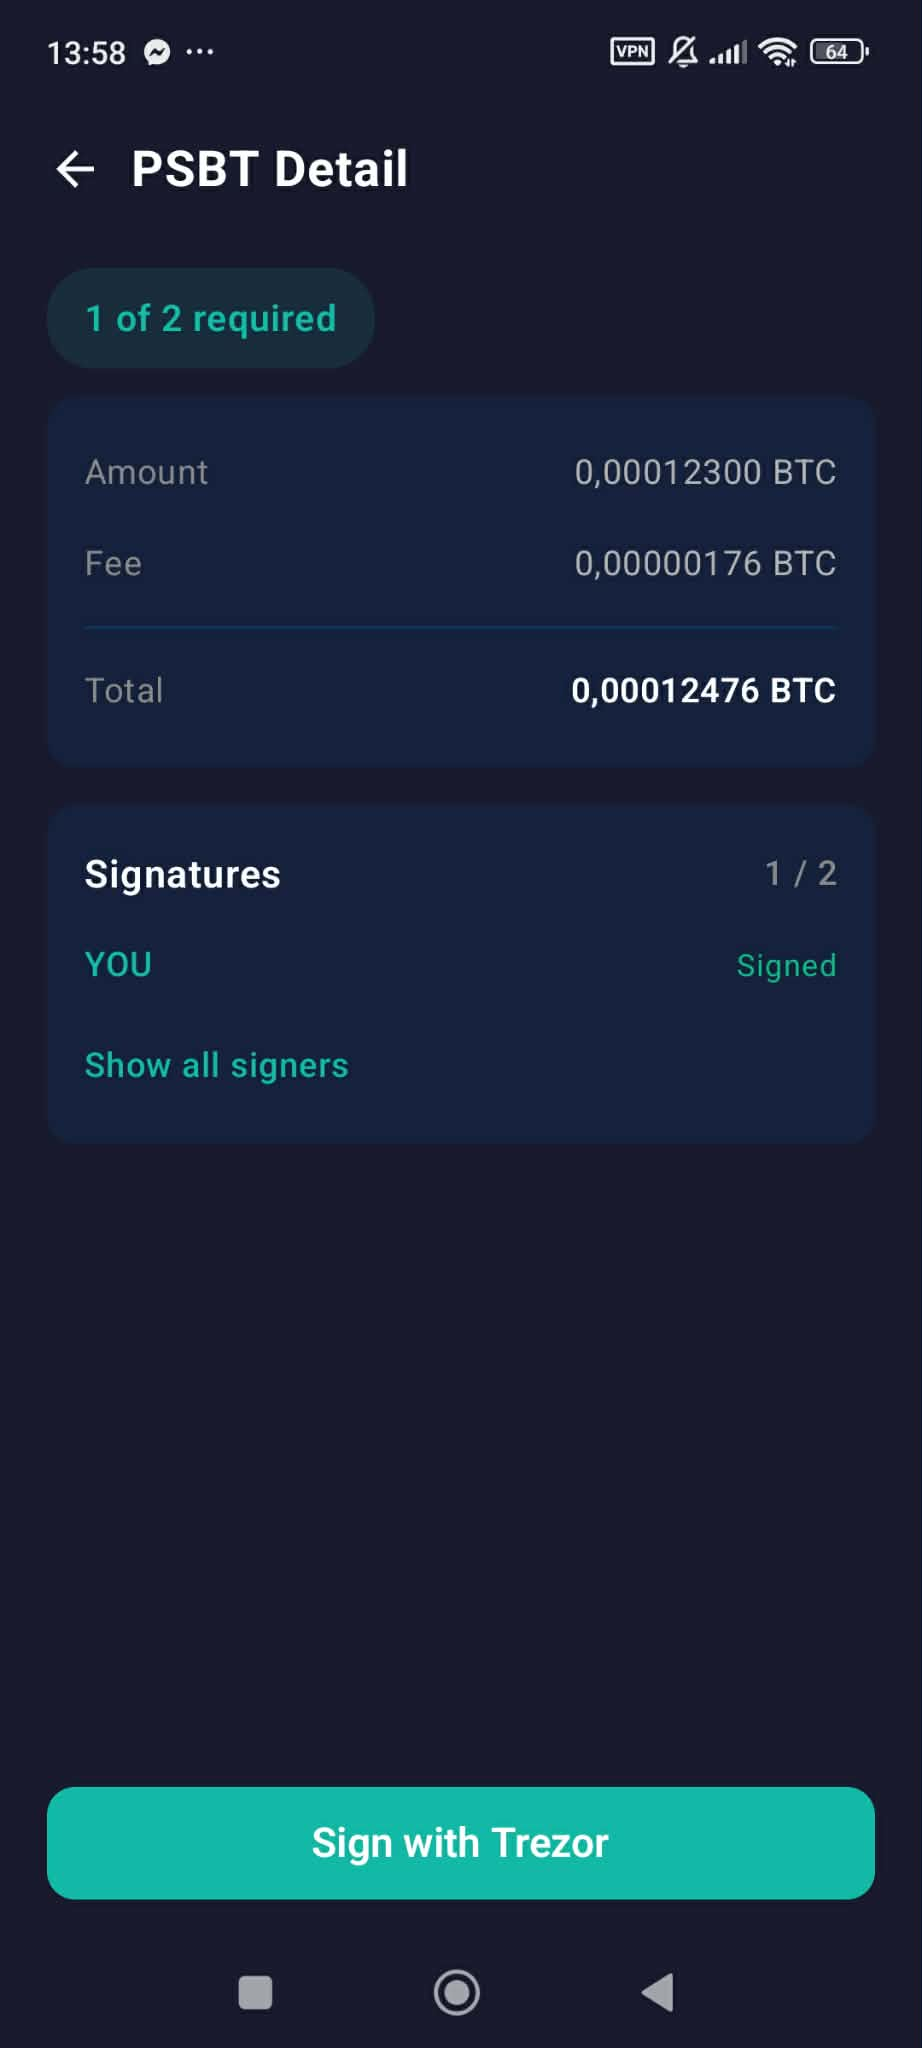
\includegraphics[height=0.22\textheight]{img/screen-psbt-detail.jpeg}\hfill
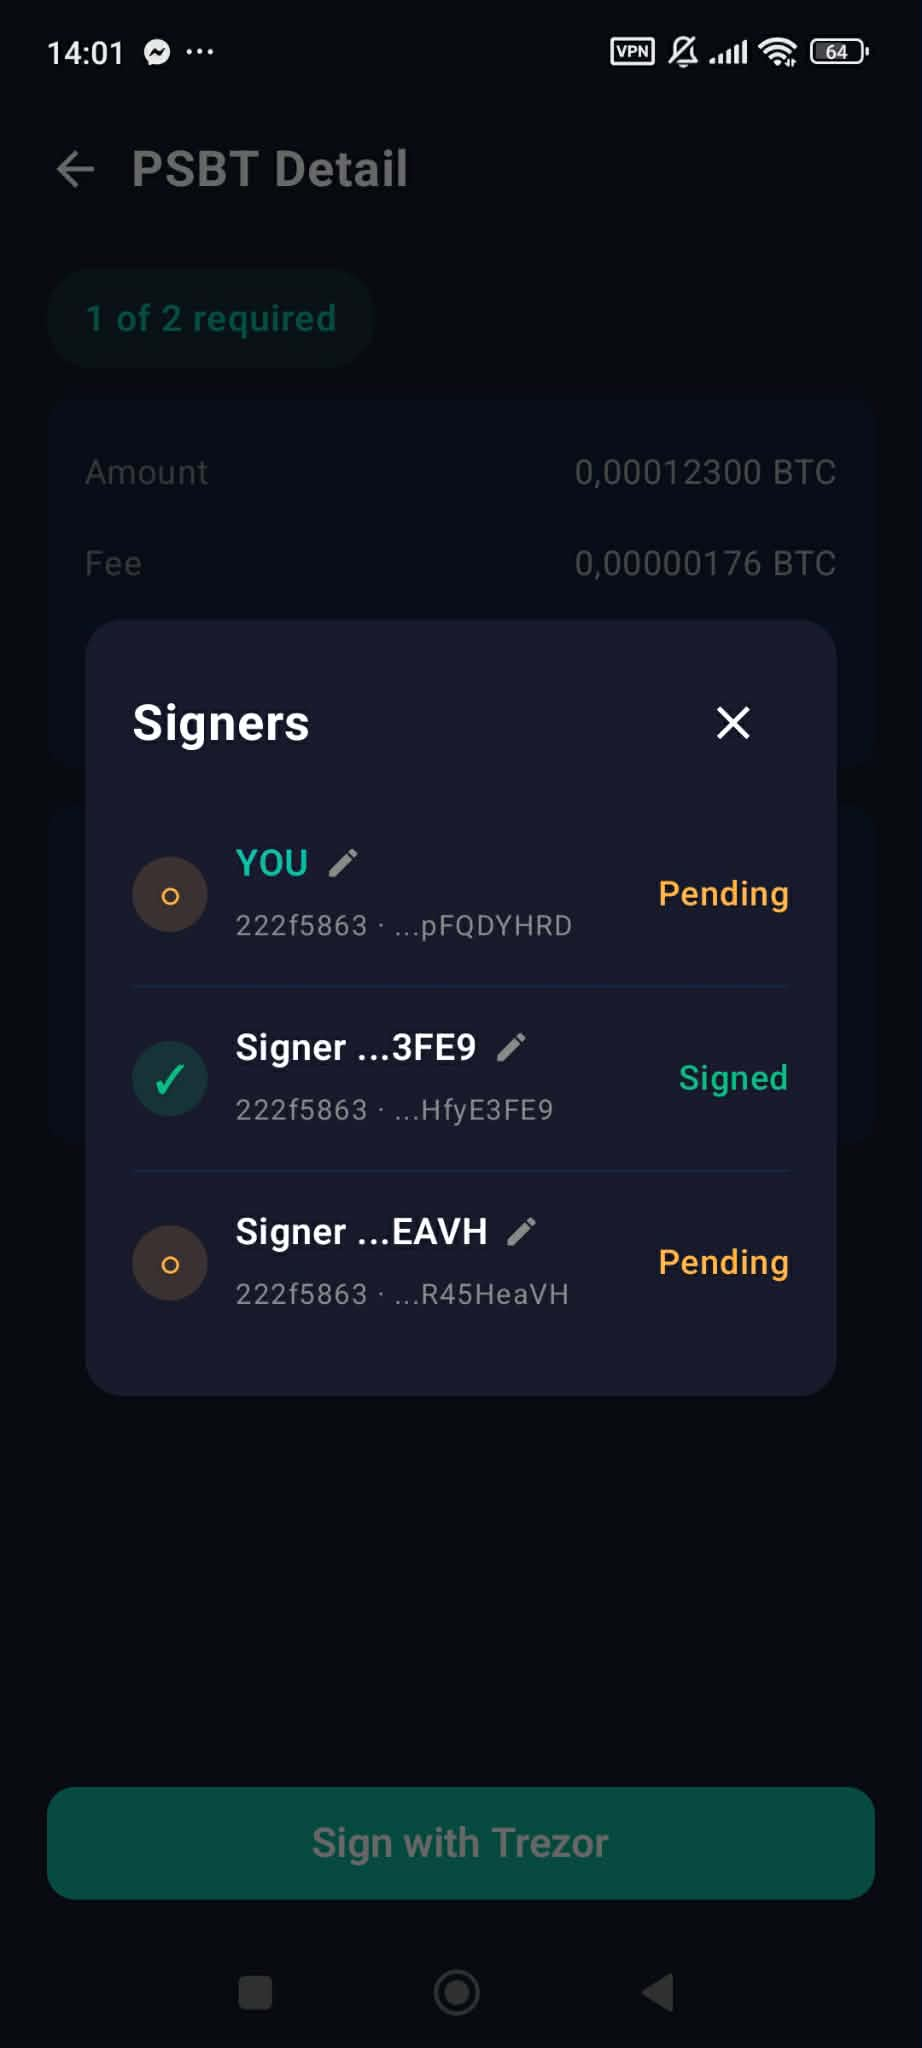
\includegraphics[height=0.22\textheight]{img/screen-psbt-signers.jpeg}\hfill
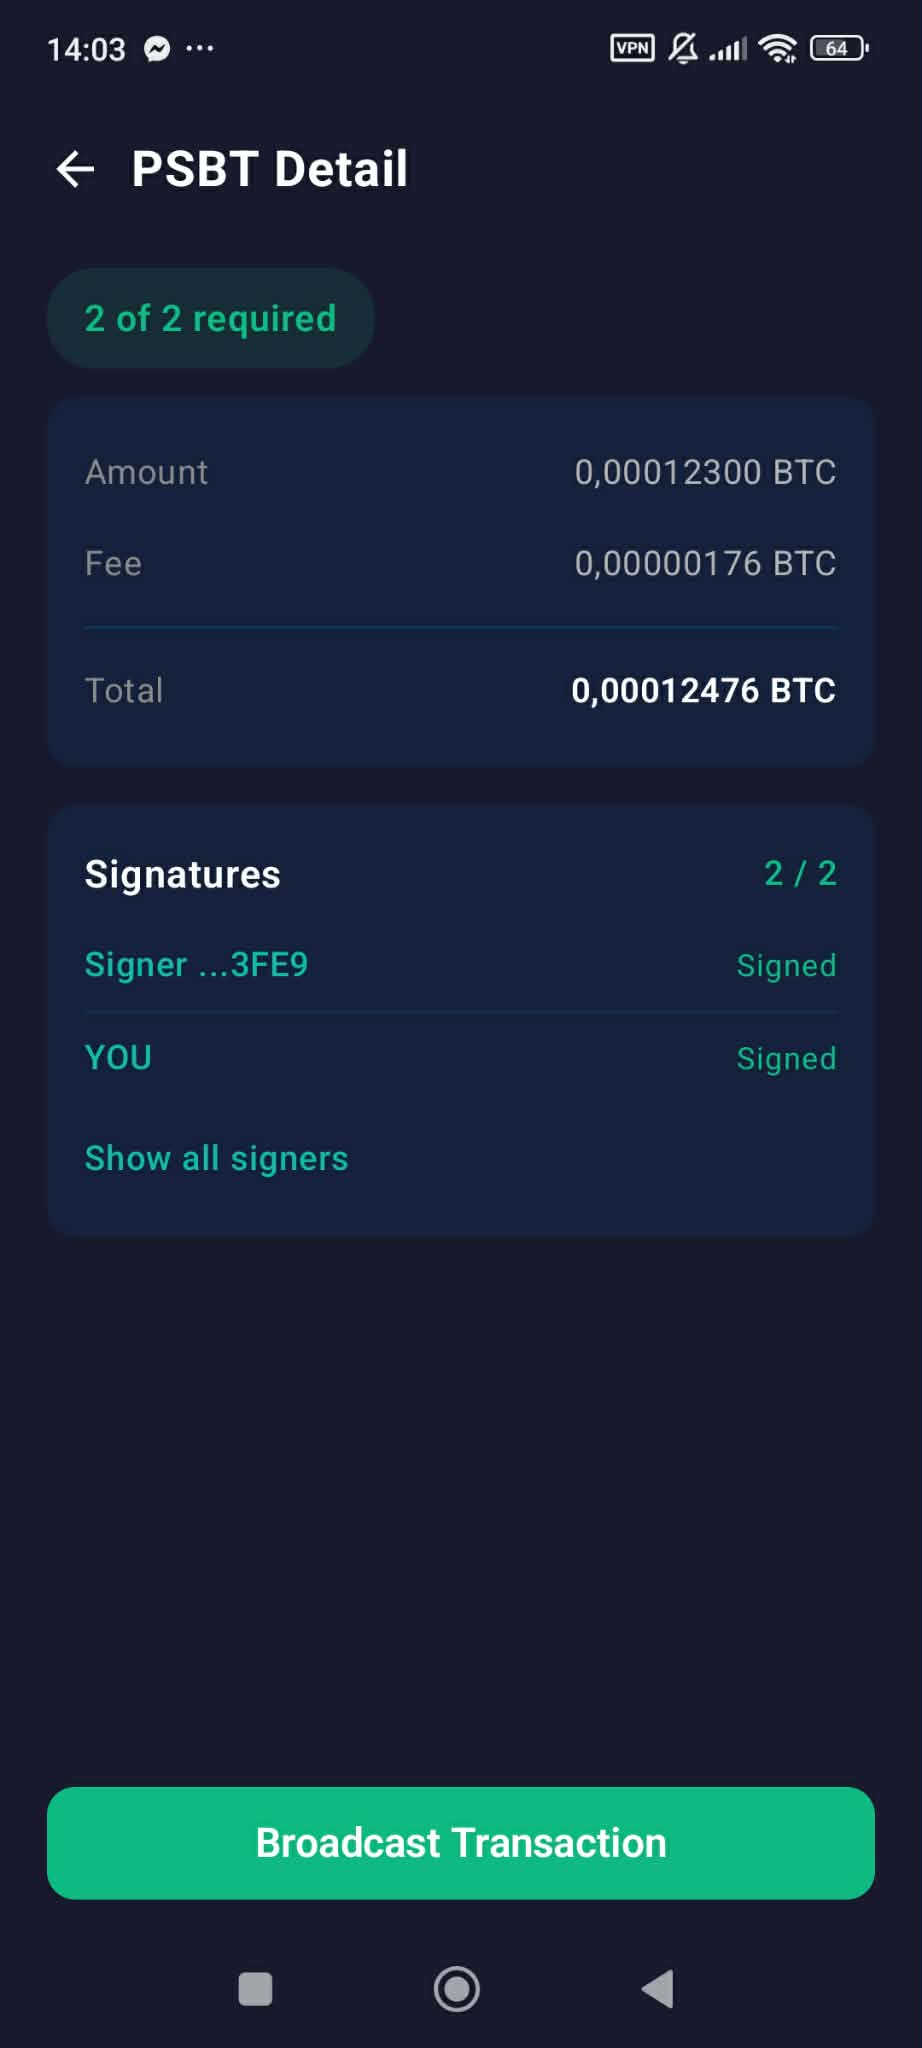
\includegraphics[height=0.22\textheight]{img/screen-psbt-broadcast.jpeg}
\caption[PSBT workflow]{PSBT workflow. Zleva: seznam PSBT transakcí;
detail PSBT bezprostředně po vytvoření (0 ze~2 podpisů) s~tlačítkem
\emph{Cancel PSBT} pro stažení návrhu před podpisem; dialog signerů
se stavy Signed~/~Pending a~příznakem \emph{YOU}; PSBT s~dosaženým
prahem (2 ze~2) připravené k~broadcastu.}
\label{fig:screen-psbt-flow}
\end{figure}

\textbf{Detail PSBT.}
Po kliknutí na konkrétní PSBT se otevře detailní obrazovka
(obrázek~\ref{fig:screen-psbt-flow}, uprostřed) se souhrnem částky,
poplatku a~celkové hodnoty transakce. Klíčovou součástí je přehled
podpisů -- barevný indikátor zobrazuje aktuální stav (například
\uv{1 of~2 required}) a~pod ním je seznam cosignerů s~informací, zda
každý z~nich již podepsal.

V~dialogu signerů (obrázek~\ref{fig:screen-psbt-flow}, vpravo, přístupném
přes odkaz \emph{Show all signers}) uživatel vidí u~každého cosignera jeho
stav, fingerprint a~zkratku veřejného klíče. Cosignerům je možné přiřadit
pojmenování (například \uv{Pepa}) stisknutím ikony tužky -- název se uloží
pouze pro aktuálně přihlášené zařízení a~ostatním cosignerům se nezobrazí,
aby osobní poznámky neprosakovaly mezi členy sdílené peněženky. Cosigner
odpovídající aktuálně přihlášenému účtu je označen příznakem \emph{YOU}.

Pokud transakce čeká na podpis aktuálního cosignera, zobrazí se tlačítko
\emph{Sign with Trezor}, které přesměruje uživatele do Trezor Suite Mobile.
Po stisknutí tlačítko zšedne a~popisek odráží aktuální fázi
(\emph{Waiting for Trezor\ldots} během čekání na callback,
\emph{Processing\ldots} při následném odesílání podpisů na backend),
což brání opakovanému spuštění deeplinku.
Návrh transakce, který ještě nebyl odeslán do sítě, lze tlačítkem
\emph{Cancel PSBT} stáhnout -- backend záznam smaže a~uvolní zarezervované
UTXO zpět k~použití v~jiné transakci. Po dobu čekání na Trezor se Cancel PSBT
skrývá a~místo něj se zobrazí nedestruktivní \emph{Cancel signing}, které
pouze ukončí čekání, aniž by draft smazalo -- případný pozdě dorazivší
podpis tak nepadne na neexistující záznam. Po broadcastu obě tlačítka mizí,
aby zůstal zachován audit záznam již odeslaných transakcí.

\textbf{Doplnění podpisu dalším cosignerem.}
Pro doplnění dalšího podpisu musí podepsat jiný cosigner. V~reálném nasazení
si druhý cosigner otevře tutéž transakci ve své vlastní instanci aplikace
napojené na společný backend; pro účely testování (kdy máme jeden Trezor
a~tři účty na něm) lze v~jedné instanci přepnout aktivní účet v~nastavení
pod položkou \emph{Switch Account}. Po přepnutí najde uživatel
rozpracovanou transakci v~seznamu PSBT u~odpovídající multisig peněženky,
otevře její detail a~stiskne \emph{Sign with Trezor} -- aplikace ho opět
přesměruje do Trezor Suite Mobile.

Po dosažení prahu~$M$ (obrázek~\ref{fig:screen-psbt-flow}, vpravo)
má PSBT kompletní sadu podpisů. Na~detailu PSBT zmizí tlačítko
\emph{Sign with Trezor} a~místo něj se objeví \emph{Broadcast
Transaction}. Po~jeho stisknutí aplikace zavolá na~backend endpoint
pro~broadcast, ten výslednou transakci propaguje přes
\texttt{blockchain-service} do~Bitcoinové sítě a~aplikace zobrazí
potvrzení s~identifikátorem transakce shodně jako u~singlesig
odeslání. Broadcast je tedy vždy explicitní akcí některého
cosignera na~detailu PSBT -- po~přijetí posledního podpisu se
transakce sama od~sebe neodesílá.

\textbf{Zrušení rozpracované transakce.} Pokud uživatel zjistí, že
transakce byla vytvořena s~chybnými parametry (například špatná
cílová adresa nebo částka), nebo cosigner z~jakéhokoli důvodu
nepodepíše, nabízí detail PSBT tlačítko \emph{Cancel PSBT}. Po
potvrzení v~dialogu aplikace zavolá \texttt{DELETE /psbt/\{id\}},
backend záznam smaže a~uvolní rezervaci utracených UTXO, takže je lze
znovu použít v~nové transakci. Tlačítko je dostupné jen u~PSBT, které
ještě nebyly broadcastnuty -- broadcastované transakce se uchovávají
jako auditní stopa. Bez této možnosti by opuštěná multisig konfigurace
držela své UTXO blokované až do automatického úklidu po~sedmi dnech
(viz sekci~\ref{sec:datovy-model}).
